%%%%%%%%%%%%%%%%%%%%%%%%%%%%%%%%%%%%%%%%%
% Beamer Presentation
% LaTeX Template
% Version 1.0 (10/11/12)
%
% This template has been downloaded from:
% http://www.LaTeXTemplates.com
%
% License:
% CC BY-NC-SA 3.0 (http://creativecommons.org/licenses/by-nc-sa/3.0/)
%
%%%%%%%%%%%%%%%%%%%%%%%%%%%%%%%%%%%%%%%%%

%----------------------------------------------------------------------------------------
%	PACKAGES AND THEMES
%----------------------------------------------------------------------------------------

\documentclass{beamer}

\mode<presentation> {

% The Beamer class comes with a number of default slide themes
% which change the colors and layouts of slides. Below this is a list
% of all the themes, uncomment each in turn to see what they look like.

%\usetheme{default}
%\usetheme{AnnArbor}
%\usetheme{Antibes}
%\usetheme{Bergen}
%\usetheme{Berkeley}
%\usetheme{Berlin}
%\usetheme{Boadilla}
%\usetheme{CambridgeUS}
%\usetheme{Copenhagen}
%\usetheme{Darmstadt}
%\usetheme{Dresden}
%\usetheme{Frankfurt}
%\usetheme{Goettingen}
%\usetheme{Hannover}
%\usetheme{Ilmenau}
%\usetheme{JuanLesPins}
%\usetheme{Luebeck}
\usetheme{Madrid}
%\usetheme{Malmoe}
%\usetheme{Marburg}
%\usetheme{Montpellier}
%\usetheme{PaloAlto}
%\usetheme{Pittsburgh}
%\usetheme{Rochester}
%\usetheme{Singapore}
%\usetheme{Szeged}
%\usetheme{Warsaw}

% As well as themes, the Beamer class has a number of color themes
% for any slide theme. Uncomment each of these in turn to see how it
% changes the colors of your current slide theme.

%\usecolortheme{albatross}
%\usecolortheme{beaver}
%\usecolortheme{beetle}
%\usecolortheme{crane}
%\usecolortheme{dolphin}
%\usecolortheme{dove}
%\usecolortheme{fly}
%\usecolortheme{lily}
%\usecolortheme{orchid}
%\usecolortheme{rose}
%\usecolortheme{seagull}
%\usecolortheme{seahorse}
%\usecolortheme{whale}
%\usecolortheme{wolverine}

%\setbeamertemplate{footline} % To remove the footer line in all slides uncomment this line
%\setbeamertemplate{footline}[page number] % To replace the footer line in all slides with a simple slide count uncomment this line

%\setbeamertemplate{navigation symbols}{} % To remove the navigation symbols from the bottom of all slides uncomment this line
}
\usepackage{romannum}
\usepackage{setspace}
\usepackage{tipa}
\usepackage{graphicx} % Allows including images
\usepackage{booktabs} % Allows the use of \toprule, \midrule and \bottomrule in tables
\usepackage{pgfplots}


\pgfplotsset{select coords between index/.style 2 args={
    x filter/.code={
        \ifnum\coordindex<#1\def\pgfmathresult{}\fi
        \ifnum\coordindex>#2\def\pgfmathresult{}\fi
    }
}}
\pgfplotsset{major grid style={dotted,black!50}}
\definecolor{mycolor1}{RGB}{215,25,28}
\definecolor{mycolor2}{RGB}{253,174,97}
\definecolor{mycolor3}{RGB}{51,160,44}
\definecolor{mycolor4}{RGB}{44,123,182}
%----------------------------------------------------------------------------------------
%	TITLE PAGE
%----------------------------------------------------------------------------------------

\title[Accents 17 Presentation]{ Weighing Segmental/Syllable Errors in Foreign Accent} % The short title appears at the bottom of every slide, the full title is only on the title page

\author{Zhiyan Gao \& Steven Weinberger} % Your name
\institute[GMU] % Your institution as it will appear on the bottom of every slide, may be shorthand to save space
{
George Mason University \\ % Your institution for the title page
\medskip
\textit{Accents 2017} % Your email address
}
\date{Dec.2 2017} % Date, can be changed to a custom date




\begin{document}

\begin{frame}
\titlepage % Print the title page as the first slide
%\textsubscript{Committee:}\linebreak
%\textsubscript{Steven Weinberger, PhD}\linebreak
%\textsubscript{Douglas Wulf, PhD}\linebreak
%\textsubscript{Dennis Perzanowski, PhD}
\end{frame}

%\begin{frame}
%\frametitle{Overview} % Table of contents slide, comment this block out to remove it
%\tableofcontents % Throughout your presentation, if you choose to use \section{} and \subsection{} commands, these will automatically be printed on this slide as an overview of your presentation
%\end{frame}

%----------------------------------------------------------------------------------------
%	PRESENTATION SLIDES
%----------------------------------------------------------------------------------------

%------------------------------------------------
\section{Introduction}
\begin{frame}
\frametitle{Introduction}
\begin{enumerate}
\onslide<1->{\item {\bf Foreign Accent}}\linebreak\linebreak
\onslide<2->\textit{The {\bf perceivable} deviation of non-native speech from the native speech norm is often defined as “foreign accent”.\linebreak\textsubscript {(Munro \& Derwing, 1998)} }\linebreak
\linebreak
\onslide<3->{\item {\bf Accentedness Perception}}\linebreak\linebreak
\onslide<4->\textit{Native speakers can detect foreign accent even in very short L2 speech samples}\linebreak\textsubscript{30ms-long stimuli (Flege,1984), ERP N100 (Steinschneider et. al., 1999)}
\end{enumerate}
\end{frame}

\section{Research Questions} % Sections can be created in order to organize your presentation into discrete blocks, all sections and subsections are automatically printed in the table of contents as an overview of the talk
%------------------------------------------------

%\subsection{Subsection Example} % A subsection can be created just before a set of slides with a common theme to further break down your presentation into chunks
\begin{frame}
\frametitle{Research Questions}
\begin{spacing}{2}
\begin{enumerate}
\onslide<1->{\item What are the segmental/structural attributes of {\bf foreign accent}?}
\onslide<2->{\item Do some L2 speech errors contribute more to accent than others?}
%\onslide<3->{\item Why some L2 errors are more accented than others?}
\end{enumerate}
\end{spacing}
\end{frame}


\section{Background}
\subsection{L2 errors that affect accentedness}
\begin{frame}
\frametitle{Background \Romannum{1}:L2 Errors}
\begin{itemize}
\onslide<1->{\item Consonant errors affect accentedness \linebreak
\textit{VOT, Liquids \linebreak \textsubscript{(Gonzalez-Bueno,1997; Solon,2015)}}\linebreak}
\onslide<2->{\item Vowels are complicated \linebreak
\textit{Duration, Formats, Vowel space \textsubscript{(Major, 1987;McCullough,2013;Chan, Hall, and Assgari,2016)}}\linebreak}
\onslide<3->{\item What about syllables?\linebreak
\textit{Segment Insertion, Segment Deletion \linebreak\textsubscript{(Magen, 1998; Van Den Doel, 2006)}}}
\end{itemize}
\end{frame}


\subsection{The degree of accentedness}
%Magen(1998)
\begin{frame}
\frametitle{Background \Romannum{2}: the Ranking of Errors}
\onslide<1->{\begin{block}{Magen (1998):speaker 1}
Epenthetic schwa, -ed ending, {\bf tense-lax}, final/s/, \textipa{tS} to \textipa{S}, lexical and phrasal stress\linebreak  $>>$ \linebreak\
Stop voicing,/s/ to /z/, vowel reduction 
\end{block}
}
\onslide<2->{\begin{block}{Magen (1998):speaker 2}
Epenthetic schwa, final/s/, \textipa{tS} to \textipa{S}, lexical and phrasal stress\linebreak  $>>$ \linebreak
Stop voicing,/s/ to /z/, vowel reduction, {\bf tense-lax}
\end{block}
}
\end{frame}
%Doel(2006)
\begin{frame}
\frametitle{Background \Romannum{2}: the Ranking of Errors}
\onslide<1->{\begin{block}{Van Den Doel (2006): 222 American Listeners}
Lexical Stress, Uvular-r $>>$\linebreak\linebreak
Voicing, Epenthesis in /lm/, /w/ to /v/, /\textipa{\ae}/ to /e/ $>>$ \linebreak\linebreak
Coda weakening in "off" and "that" $>>$ \linebreak\linebreak
VOT shortening on /t\super h/,/\textipa{2}/ to /\textipa{A}/,intonation $>>$ \linebreak\linebreak
yod-insertion in "news"
\end{block}
}
\end{frame}
%Gao(2016)
\begin{frame}
\begin{itemize}
\frametitle{Background \Romannum{2}: Limitations}
\onslide <1->{\item Errors were artifically created/F0 contours were synthesized}
\onslide <2->{\item Each stimulus may contain multiple errors}
\onslide <3->{\item Phonological Environment was not well controlled}
\end{itemize}
\end{frame}
%------------------------------------------------------------------------

%-------------------------------------------
\section{The Current Study}
\subsection{overview}
\begin{frame}
\frametitle{The current study \Romannum{1}: Aims}
\begin{enumerate}
\item{Design a perception study to obtain accentedness ratings;}\linebreak
\item{Rank the L2 errors by accentedness;}\linebreak
\end{enumerate}
\end{frame}

%------------------------------------------------
\subsection{Research design}
\begin{frame}
\frametitle{The current study \Romannum{1}: Research Design}
Stimuli:
\begin{itemize} 
\item 1 error per stimulus
\item A variety of  errors'
\item No prosody manipulation 
\end{itemize}

\end{frame}
%------------------------------------------------
\begin{frame}
\frametitle{The current study \Romannum{1}: Research Design}
Stimuli collection: \linebreak
Natural speech samples from the Speech Accent Achieve (Weinberger, 2016)
\begin{columns}[c] % The "c" option specifies centered vertical alignment while the "t" option is used for top vertical alignment
\column{.5\textwidth} % Left column and width
\begin{figure}
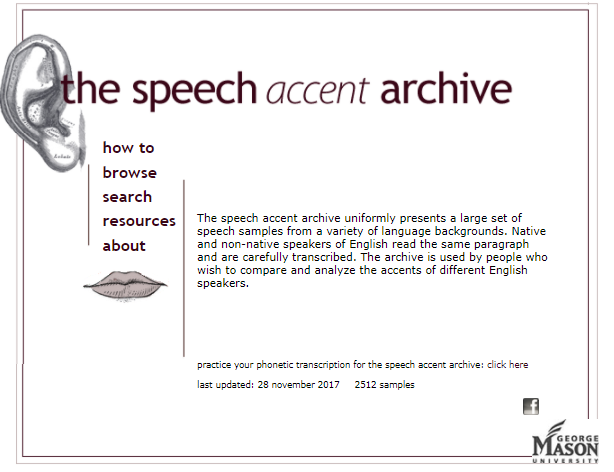
\includegraphics[width=0.8\linewidth]{accent}
\linebreak \textsubscript{accent.gmu.edu}
\end{figure}
\column{.5\textwidth} % Right column and width
\begin{figure}
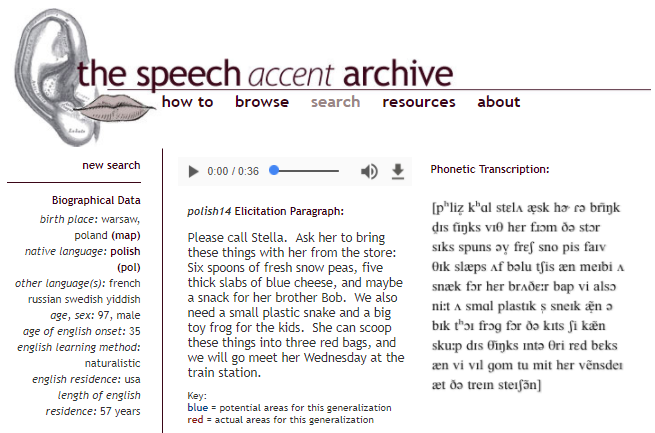
\includegraphics[width=0.8\linewidth]{saademo}
%\linebreak \textsubscript{transcriber.accent.gmu.edu}
\end{figure}
\end{columns}
\end{frame}
%-----------------------------------------------

\subsection{Stimuli Examples}
\begin{frame}
\frametitle{The current study \Romannum{1}: Research Design}
Stimuli Examples:\linebreak
5 phrases, 4 conditions, 5 tokens per phrase per condition.  100 stimuli in total. \linebreak
All stimli are L2 speech samples, representing 93 talkers and 52 different native languages.
\begin{table}
\begin{tabular}{lllll}
\toprule
& \textbf{consonant} & \textbf{vowel} & \textbf{syllable} & \textbf{correct} \\
\midrule
please call   & /\textipa{\underline{\color{red}p}li:z k\super hAl/ } & /\textipa{p\super hli:z k\super h\underline{\color{red}o}l/}&/\textipa{p\super h\underline{\color{red}@}li:z k\super hAl/} &/\textipa{p\super hli:z k\super hAl/}  \\ 
ask her       &/\textipa{\ae sk (h)@\underline{\color{red}r}}/            &/\textipa{\underline{\color{red}A}sk (h)@\*r}/        &/\textipa{\ae s\underline{ } h@\*r}/           &/\textipa{\ae sk (h)@\*r}/      \\
six spoons    &\textipa{/sIks spun\underline{\color{red}S}/ }             &\textipa{/s\underline{\color{red}i}ks spunz/ }         &\textipa{/sIks \underline{\color{red}@}spunz/ }            &\textipa{/sIks spunz/ }        \\
five thick    &/\textipa{faIv \underline{\color{red}t}Ik}/            &/\textipa{f\underline{\color{red}a }v TIk}/        & /\textipa{faIv\underline{\color{red}@} TIk}/          & /\textipa{faIv TIk}/        \\
small plastic &/\textipa{smO\underline{\color{red}\:l}}           &/\textipa{smOl}         &/\textipa{smOl}           &/\textipa{smOl}\\
	&\textipa{p\super hl\ae stIk}	&\textipa{p\super hl\ae st\underline{\color{red}i}k}	& \textipa{p\super hl\ae s\underline{ }Ik}/	&\textipa{p\super hl\ae stIk}/  \\
\bottomrule  
\end{tabular}
\end{table}
\end{frame}
%------------------------
\begin{frame}
\frametitle{The current study \Romannum{1}: Control for Prosody}
Control prosody in the least intrusive manner.  Prosody is a {\bf CONTROLLING} variable.  
\linebreak
\linebreak
Method: Dynamic Time Warping (DTW) 
\begin{itemize}
\item No acoustic manipulation required
\item Align F0 contours of two utterances
\item Produce a DTW score which represents alignment cost
\item The bigger the DTW score, bigger the intonational difference
\end{itemize}
\begin{columns}[c] % The "c" option specifies centered vertical alignment while the "t" option is used for top vertical alignment
\column{.45\textwidth} % Left column and width
\begin{figure}
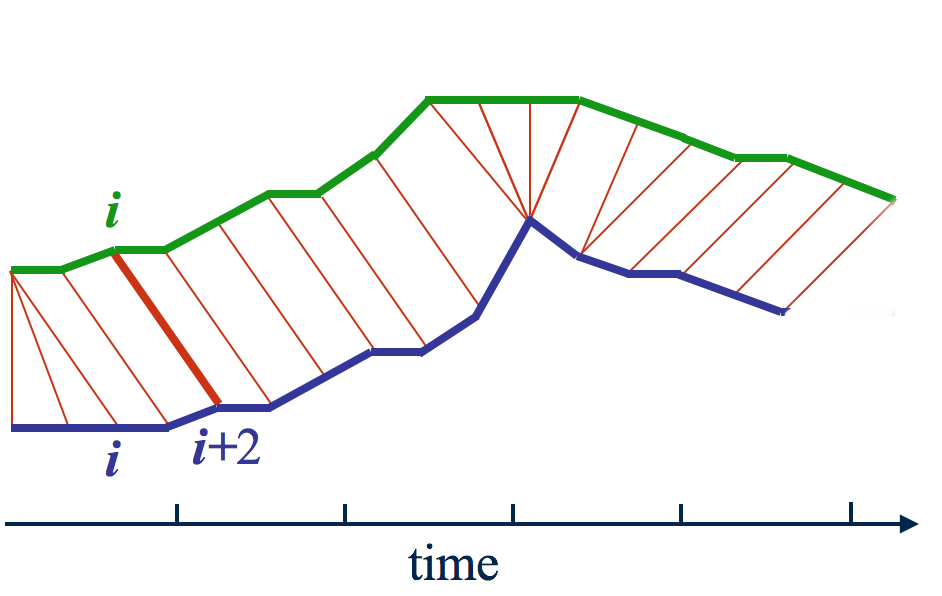
\includegraphics[width=0.8\linewidth]{dtw1}
\linebreak \textsubscript{(Tsiporkova, 2007) }
\end{figure}
\column{.55\textwidth} % Right column and width
\begin{figure}
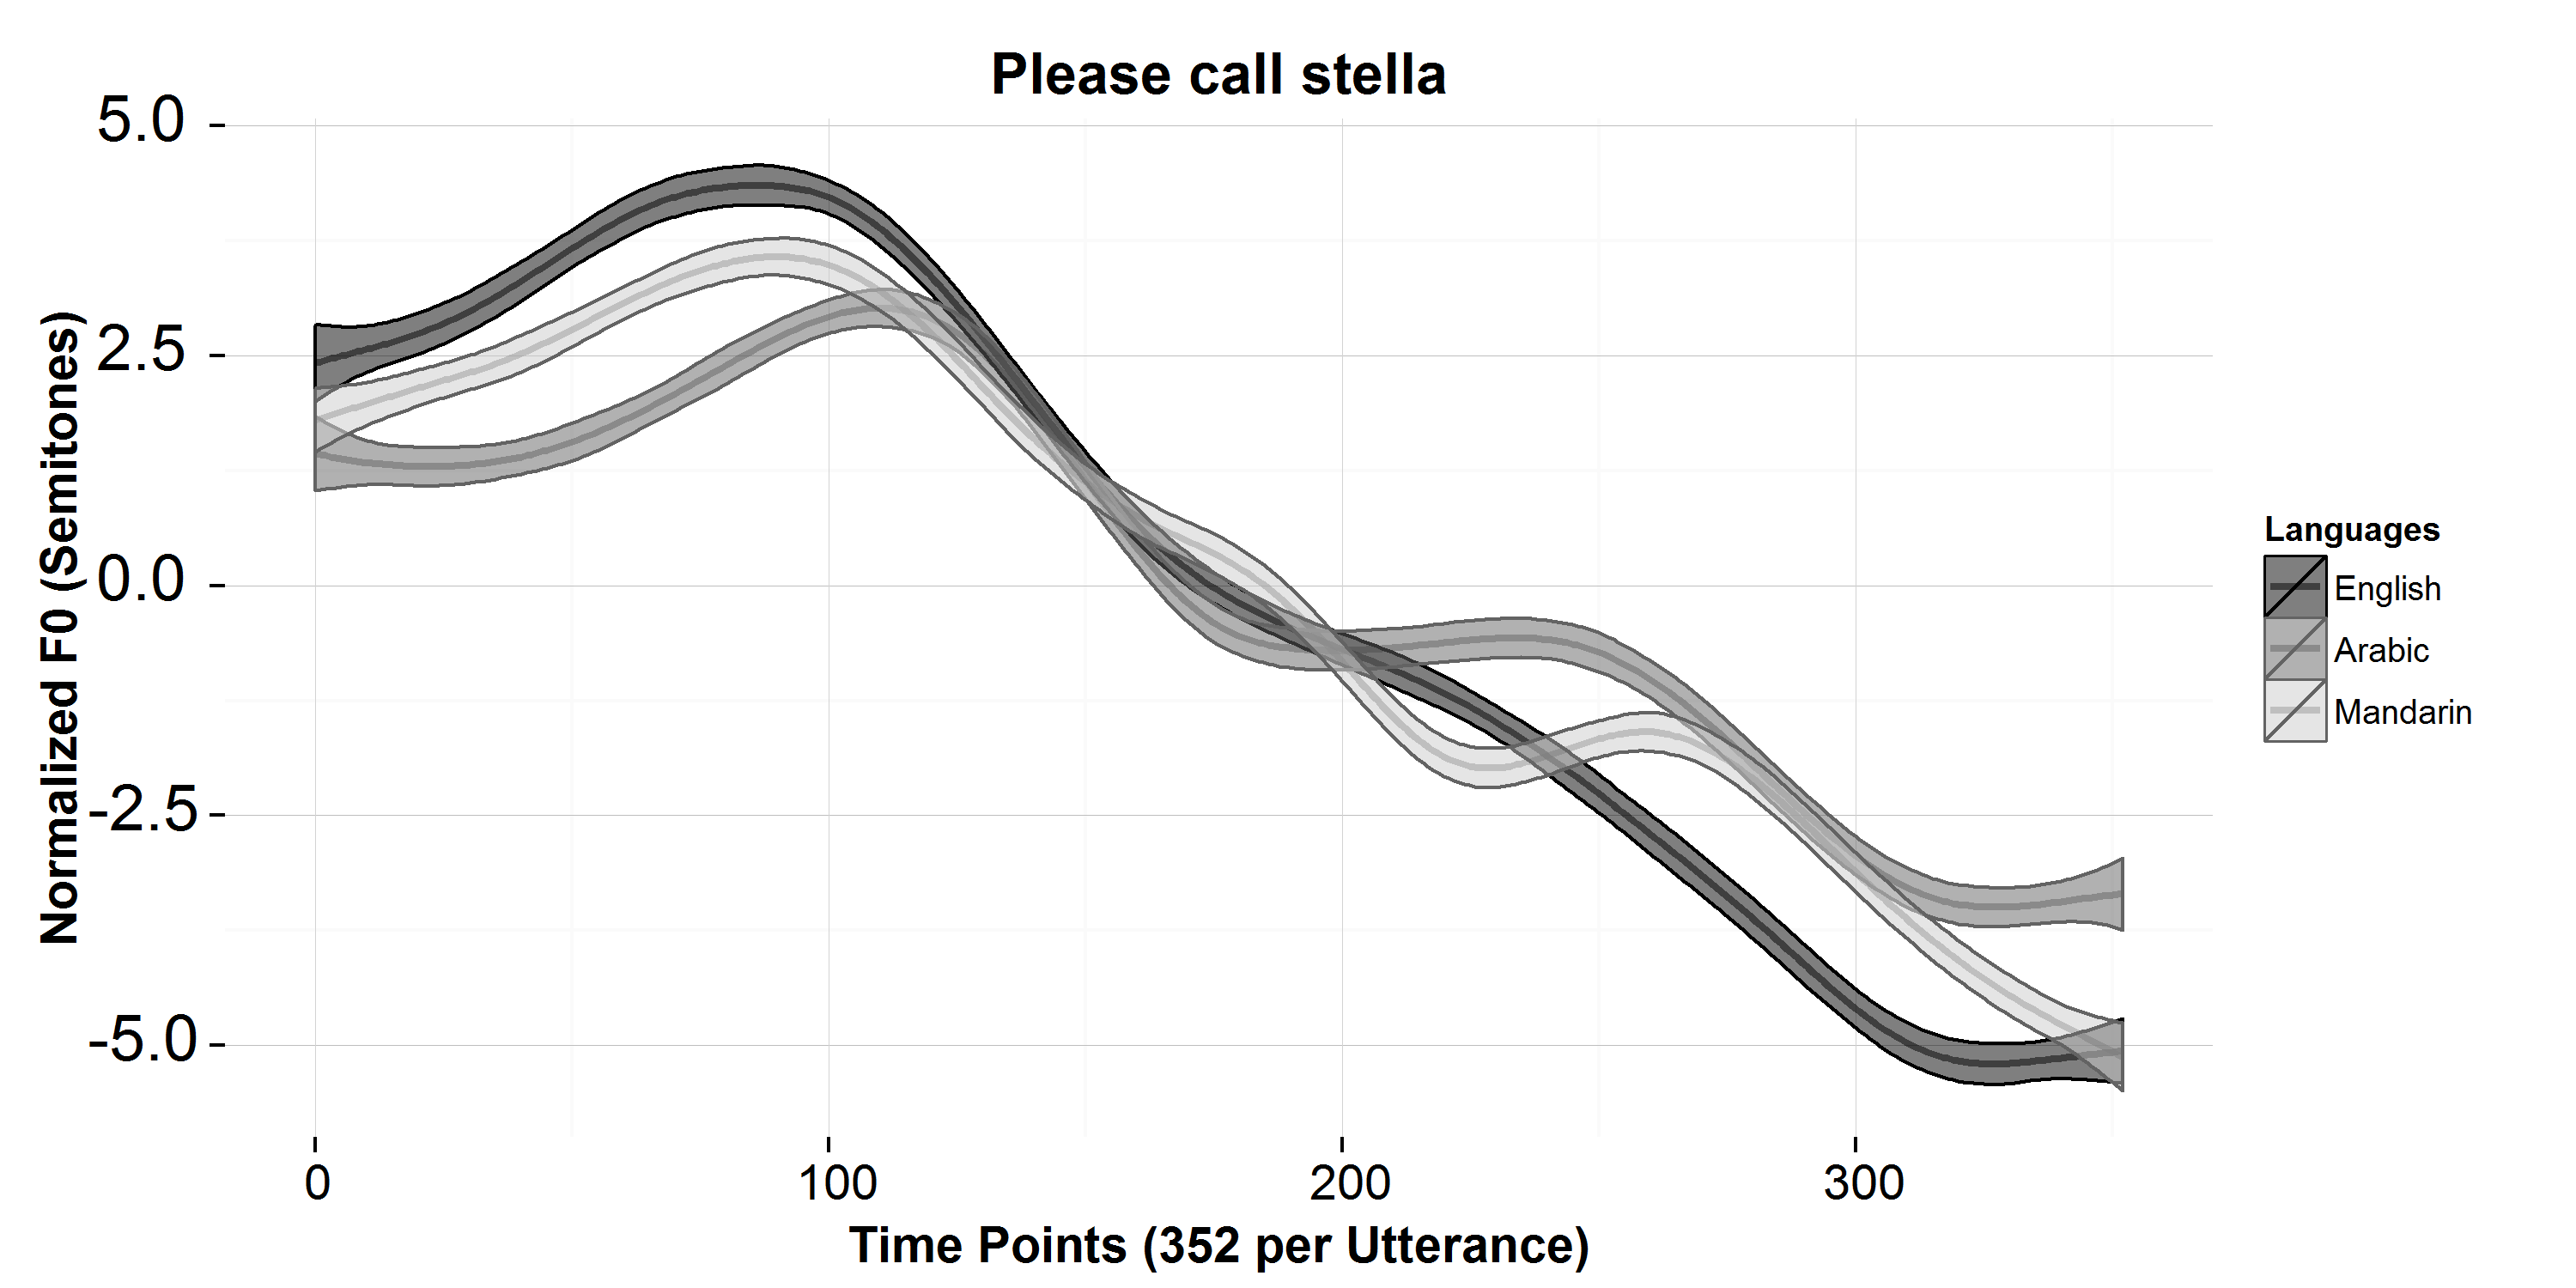
\includegraphics[width=0.9\linewidth]{dtw2}
\linebreak\textsubscript{(Morrill \& Gao,2016)}
\end{figure}
\end{columns}
\end{frame}

%------------------------------------------------
\subsection{Interface}
\begin{frame}
\frametitle{The current study \Romannum{1}: Research Design}
\begin{itemize}
\small{
\item Platform: Amazon Mechanical Turk 
\item Requirements for participants: US IPs, at least 95\%  acceptance rate.
\item Procedure:
}
\end{itemize}
\only <1>{
\begin{block}{Introduction}
\begin{figure}
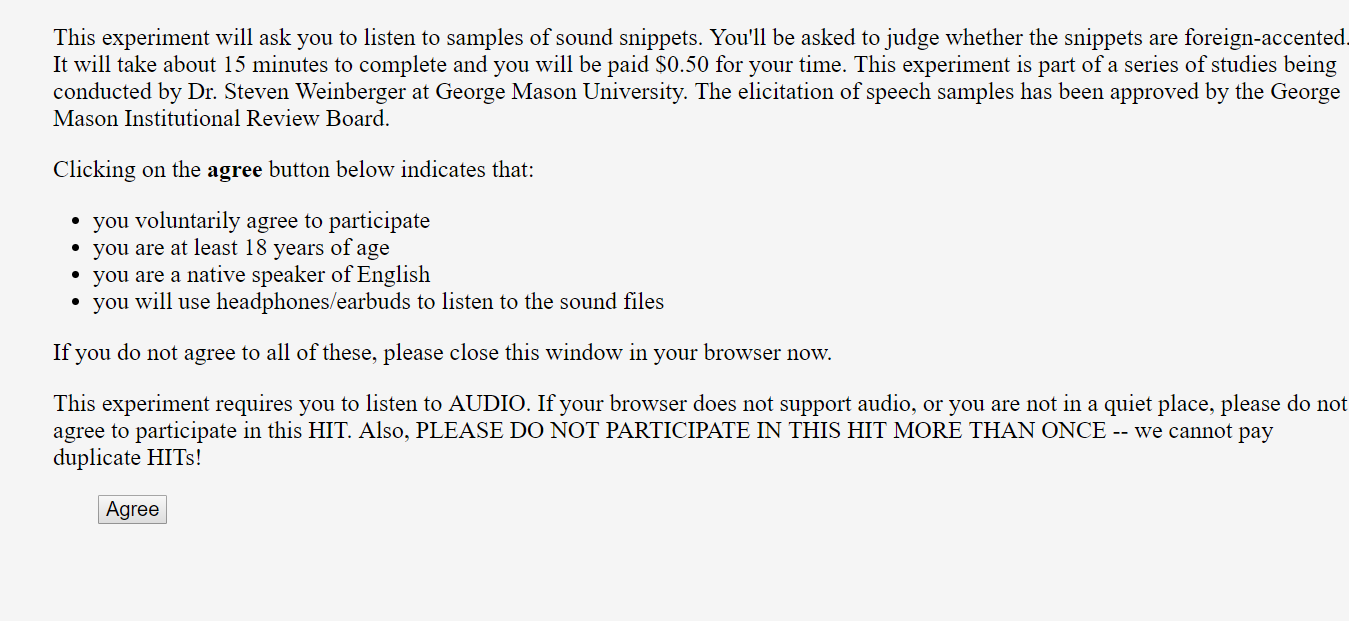
\includegraphics[width=0.8\linewidth]{demo1}
\end{figure}
\end{block}}
\only <2>{
\begin{block}{Instruction}
\begin{figure}
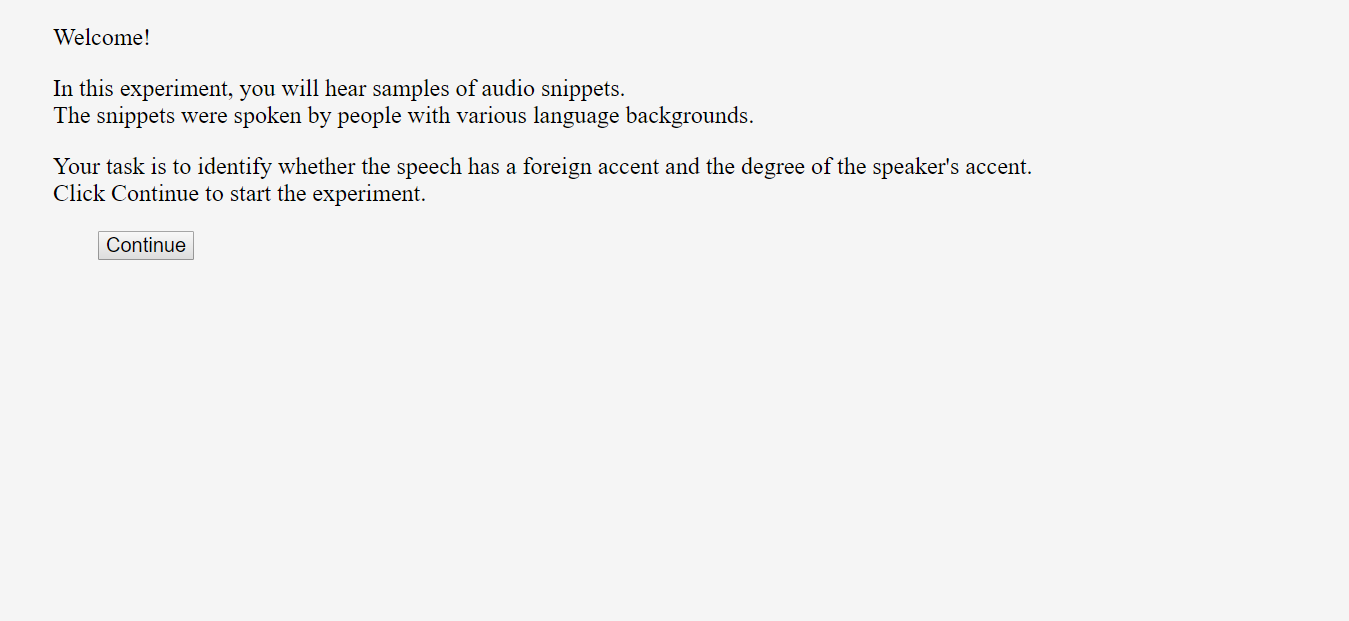
\includegraphics[width=0.8\linewidth]{demo2}
\end{figure}
\end{block}}
\only <3>{
\begin{block}{Trials:Listen to snippets (Block Randomization)}
\begin{figure}
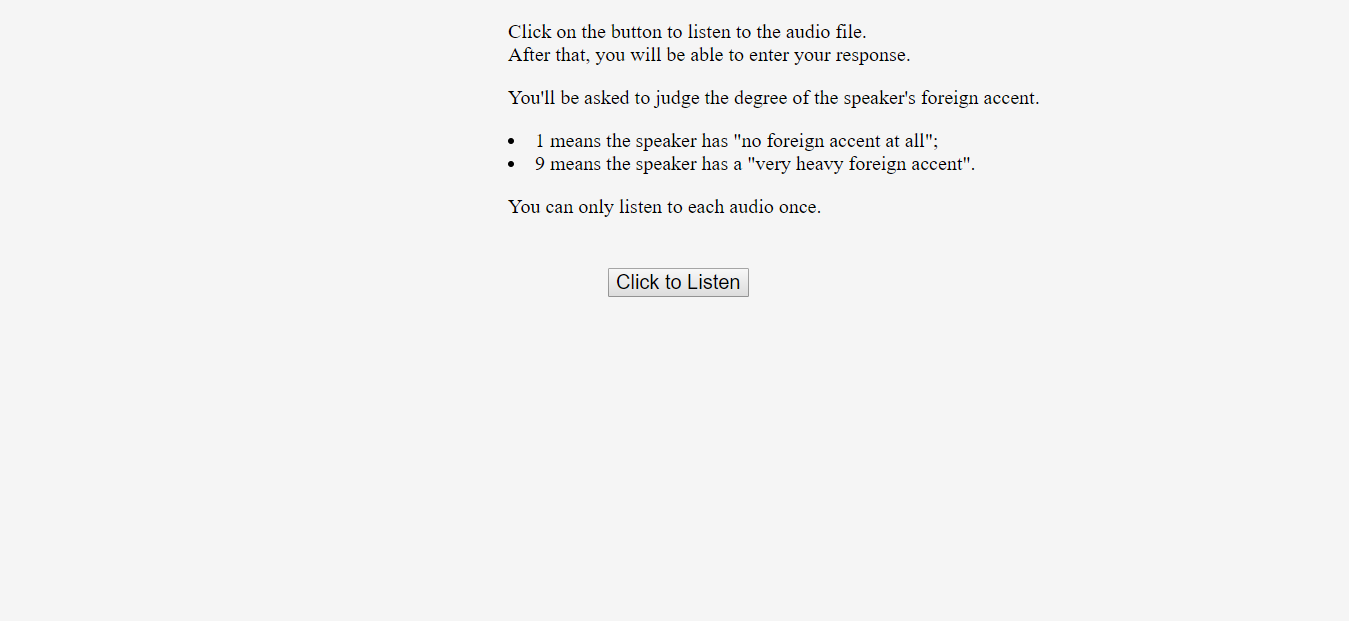
\includegraphics[width=0.8\linewidth]{demo3}
\end{figure}
\end{block}}
\only <4>{
\begin{block}{Trials:Make accentedness judgment}
\begin{figure}
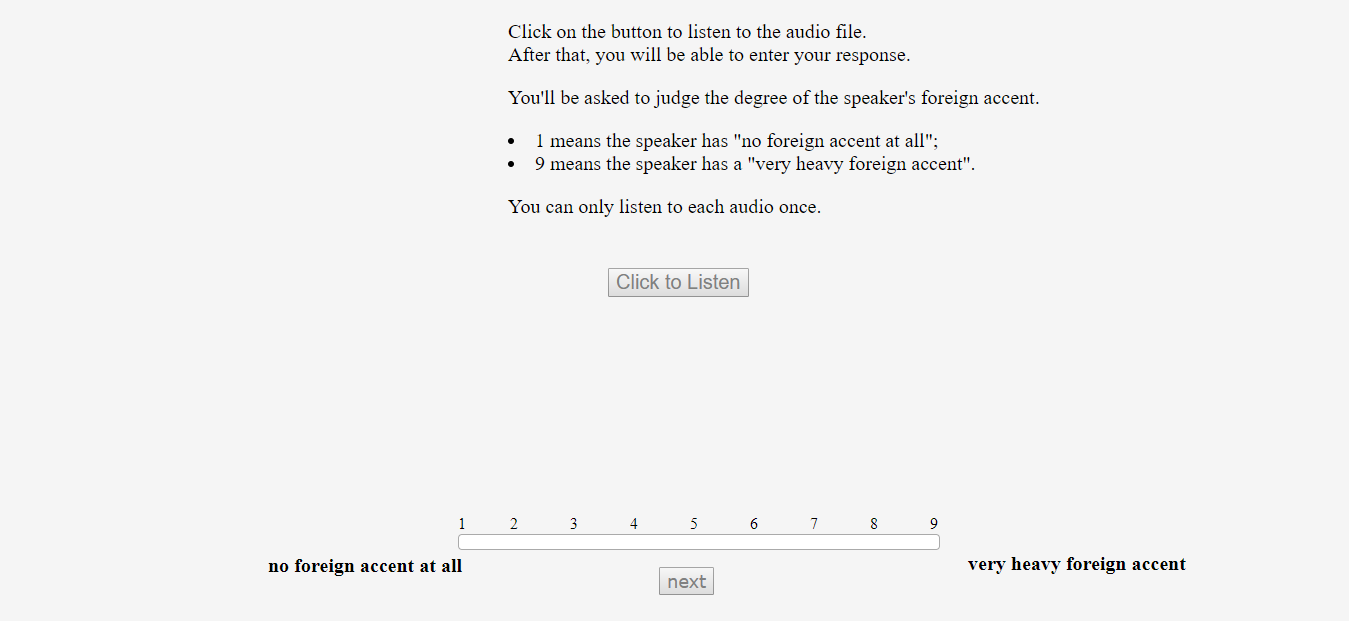
\includegraphics[width=0.8\linewidth]{demo4}
\end{figure}
\end{block}}
\only <5>{
\begin{block}{Demographics}
\begin{figure}
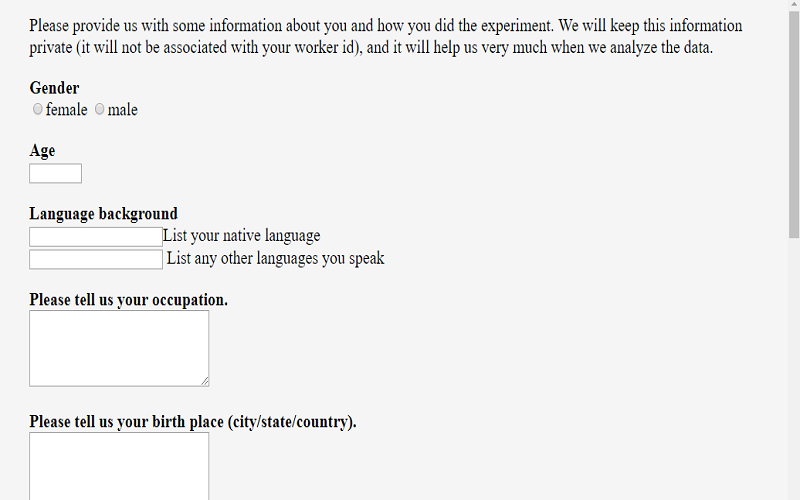
\includegraphics[width=0.8\linewidth]{demo5}
\end{figure}
\end{block}}
\end{frame}

%------------------------------------------------
\subsection{Demos of raters}
\begin{frame}
\frametitle{Rater Demographics}
\begin{itemize}
\onslide<1->{\item {110 participants, 2 reported having hearing/speech-related problem, yielding 108 participants for the analysis; all native speakers of American English}}\linebreak
\onslide<2->{\item {Male:61, Female:45, 2 did not report}}\linebreak
\onslide<3->{\item {Age: range 20-66 (M=33.50, SD=12.51)}}\linebreak
\onslide<4->{\item {Completion Time: M=12 min 20 sec, SD=3 min 12 sec; Maximum time allowed:30 min}}
\end{itemize}
\end{frame}
%------------------
\subsection{Results}
\begin{frame}
\frametitle{The current study \Romannum{3}: Results}
\begin{block}{Meaning Ratings by Type}
\begin{center}
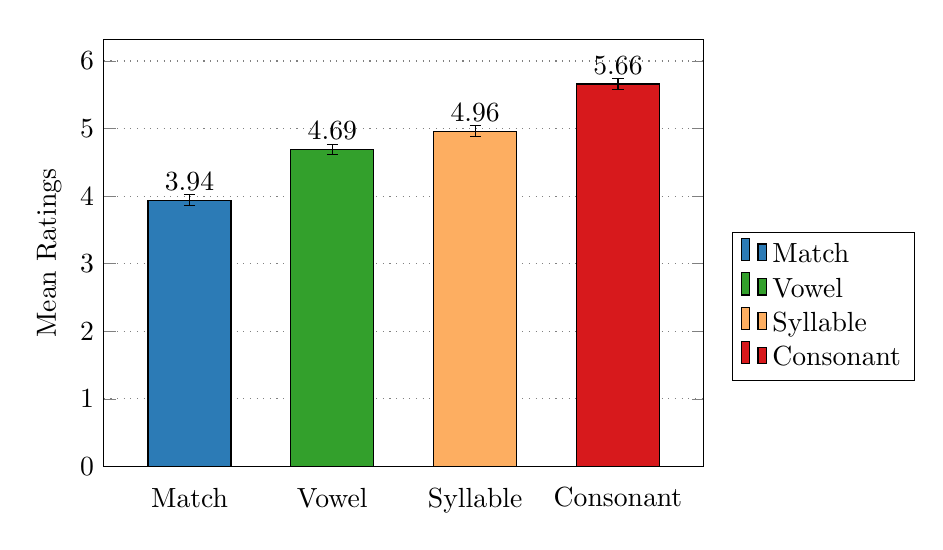
\begin{tikzpicture}
  \begin{axis}[
  ylabel={Mean Ratings},
width=9.2cm,
   height = 7cm,
    ytick distance=1,
        nodes near coords,
      major x tick style = transparent,
    ybar=3*\pgflinewidth,
      bar width=30pt,
      ymajorgrids = true,
      symbolic x coords={Match,Vowel,Syllable,Consonant},
      xtick ={Match,Vowel, Syllable, Consonant},
      scaled y ticks = false,
        legend style={at={(1.2,0.55)},
  anchor=north},
  legend cell align=left,
      enlarge x limits=0.20,
      ymin=0,
       every axis plot/.append style={
          ybar,
          bar shift=0pt,
          fill
        }
    ]
\addplot [fill=mycolor4,error bars/.cd, y dir=both, y explicit,error bar style=black] 
  coordinates {
          (Match, 3.94) += (0,0.08) -= (0,0.08)};
\addplot [fill=mycolor3,error bars/.cd, y dir=both, y explicit,error bar style=black] 
  coordinates {
          (Vowel, 4.69) += (0,0.08) -= (0,0.08)};
\addplot [fill=mycolor2,error bars/.cd, y dir=both, y explicit,error bar style=black] 
  coordinates {
          (Syllable, 4.96) += (0,0.08) -= (0,0.08)};
 \addplot [fill=mycolor1,error bars/.cd, y dir=both, y explicit,error bar style=black] 
  coordinates {
          (Consonant, 5.66) += (0,0.08) -= (0,0.08)};
 \legend{Match,Vowel,Syllable,Consonant}
 \end{axis}
\end{tikzpicture}
\end{center}


\end{block}
\end{frame}


\begin{frame}
\frametitle{The current study \Romannum{3}: Results}
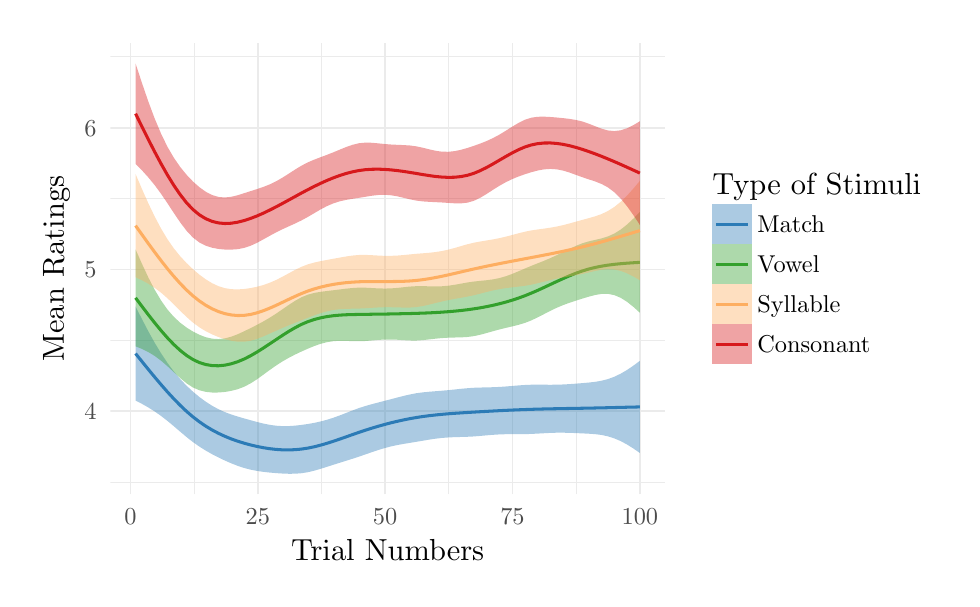
\begin{tikzpicture}[x=1pt,y=1pt]
\definecolor{fillColor}{RGB}{255,255,255}
\path[use as bounding box,fill=fillColor,fill opacity=0.00] (0,0) rectangle (334.04,199.17);
\begin{scope}
\path[clip] (  0.00,  0.00) rectangle (334.04,199.17);

\path[] (  0.00,  0.00) rectangle (334.04,199.17);
\end{scope}
\begin{scope}
\path[clip] ( 29.87, 30.56) rectangle (230.32,193.67);
\definecolor{drawColor}{gray}{0.92}

\path[draw=drawColor,line width= 0.3pt,line join=round] ( 29.87, 34.99) --
	(230.32, 34.99);

\path[draw=drawColor,line width= 0.3pt,line join=round] ( 29.87, 86.20) --
	(230.32, 86.20);

\path[draw=drawColor,line width= 0.3pt,line join=round] ( 29.87,137.41) --
	(230.32,137.41);

\path[draw=drawColor,line width= 0.3pt,line join=round] ( 29.87,188.63) --
	(230.32,188.63);

\path[draw=drawColor,line width= 0.3pt,line join=round] ( 60.15, 30.56) --
	( 60.15,193.67);

\path[draw=drawColor,line width= 0.3pt,line join=round] (106.17, 30.56) --
	(106.17,193.67);

\path[draw=drawColor,line width= 0.3pt,line join=round] (152.18, 30.56) --
	(152.18,193.67);

\path[draw=drawColor,line width= 0.3pt,line join=round] (198.20, 30.56) --
	(198.20,193.67);

\path[draw=drawColor,line width= 0.6pt,line join=round] ( 29.87, 60.59) --
	(230.32, 60.59);

\path[draw=drawColor,line width= 0.6pt,line join=round] ( 29.87,111.81) --
	(230.32,111.81);

\path[draw=drawColor,line width= 0.6pt,line join=round] ( 29.87,163.02) --
	(230.32,163.02);

\path[draw=drawColor,line width= 0.6pt,line join=round] ( 37.14, 30.56) --
	( 37.14,193.67);

\path[draw=drawColor,line width= 0.6pt,line join=round] ( 83.16, 30.56) --
	( 83.16,193.67);

\path[draw=drawColor,line width= 0.6pt,line join=round] (129.17, 30.56) --
	(129.17,193.67);

\path[draw=drawColor,line width= 0.6pt,line join=round] (175.19, 30.56) --
	(175.19,193.67);

\path[draw=drawColor,line width= 0.6pt,line join=round] (221.21, 30.56) --
	(221.21,193.67);

\path[fill=mycolor4,fill opacity=0.40] ( 38.98, 98.44) --
	( 41.29, 93.86) --
	( 43.59, 89.46) --
	( 45.90, 85.31) --
	( 48.21, 81.48) --
	( 50.51, 78.02) --
	( 52.82, 74.93) --
	( 55.13, 72.20) --
	( 57.43, 69.78) --
	( 59.74, 67.63) --
	( 62.05, 65.71) --
	( 64.35, 64.02) --
	( 66.66, 62.54) --
	( 68.97, 61.29) --
	( 71.27, 60.25) --
	( 73.58, 59.39) --
	( 75.89, 58.65) --
	( 78.19, 57.98) --
	( 80.50, 57.34) --
	( 82.81, 56.70) --
	( 85.11, 56.13) --
	( 87.42, 55.66) --
	( 89.73, 55.34) --
	( 92.03, 55.19) --
	( 94.34, 55.21) --
	( 96.65, 55.36) --
	( 98.95, 55.62) --
	(101.26, 55.96) --
	(103.57, 56.37) --
	(105.87, 56.88) --
	(108.18, 57.49) --
	(110.49, 58.23) --
	(112.79, 59.06) --
	(115.10, 59.96) --
	(117.41, 60.87) --
	(119.71, 61.71) --
	(122.02, 62.46) --
	(124.33, 63.11) --
	(126.63, 63.71) --
	(128.94, 64.31) --
	(131.25, 64.91) --
	(133.55, 65.52) --
	(135.86, 66.11) --
	(138.17, 66.64) --
	(140.47, 67.08) --
	(142.78, 67.39) --
	(145.09, 67.61) --
	(147.39, 67.80) --
	(149.70, 67.98) --
	(152.01, 68.19) --
	(154.31, 68.43) --
	(156.62, 68.68) --
	(158.93, 68.89) --
	(161.23, 69.05) --
	(163.54, 69.13) --
	(165.85, 69.19) --
	(168.15, 69.25) --
	(170.46, 69.35) --
	(172.77, 69.51) --
	(175.07, 69.70) --
	(177.38, 69.90) --
	(179.69, 70.06) --
	(181.99, 70.15) --
	(184.30, 70.17) --
	(186.61, 70.15) --
	(188.91, 70.13) --
	(191.22, 70.16) --
	(193.53, 70.24) --
	(195.83, 70.37) --
	(198.14, 70.54) --
	(200.45, 70.73) --
	(202.75, 70.93) --
	(205.06, 71.20) --
	(207.37, 71.59) --
	(209.67, 72.18) --
	(211.98, 73.03) --
	(214.29, 74.14) --
	(216.59, 75.49) --
	(218.90, 77.06) --
	(221.21, 78.78) --
	(221.21, 45.49) --
	(218.90, 47.09) --
	(216.59, 48.54) --
	(214.29, 49.78) --
	(211.98, 50.77) --
	(209.67, 51.50) --
	(207.37, 51.99) --
	(205.06, 52.28) --
	(202.75, 52.45) --
	(200.45, 52.56) --
	(198.14, 52.67) --
	(195.83, 52.76) --
	(193.53, 52.81) --
	(191.22, 52.81) --
	(188.91, 52.74) --
	(186.61, 52.62) --
	(184.30, 52.49) --
	(181.99, 52.37) --
	(179.69, 52.30) --
	(177.38, 52.29) --
	(175.07, 52.29) --
	(172.77, 52.27) --
	(170.46, 52.19) --
	(168.15, 52.05) --
	(165.85, 51.86) --
	(163.54, 51.65) --
	(161.23, 51.46) --
	(158.93, 51.34) --
	(156.62, 51.27) --
	(154.31, 51.21) --
	(152.01, 51.10) --
	(149.70, 50.92) --
	(147.39, 50.65) --
	(145.09, 50.31) --
	(142.78, 49.92) --
	(140.47, 49.53) --
	(138.17, 49.15) --
	(135.86, 48.77) --
	(133.55, 48.35) --
	(131.25, 47.85) --
	(128.94, 47.24) --
	(126.63, 46.54) --
	(124.33, 45.76) --
	(122.02, 44.96) --
	(119.71, 44.16) --
	(117.41, 43.41) --
	(115.10, 42.68) --
	(112.79, 41.96) --
	(110.49, 41.23) --
	(108.18, 40.49) --
	(105.87, 39.76) --
	(103.57, 39.09) --
	(101.26, 38.54) --
	( 98.95, 38.17) --
	( 96.65, 37.99) --
	( 94.34, 37.97) --
	( 92.03, 38.06) --
	( 89.73, 38.21) --
	( 87.42, 38.41) --
	( 85.11, 38.67) --
	( 82.81, 39.01) --
	( 80.50, 39.47) --
	( 78.19, 40.08) --
	( 75.89, 40.84) --
	( 73.58, 41.74) --
	( 71.27, 42.75) --
	( 68.97, 43.85) --
	( 66.66, 45.04) --
	( 64.35, 46.35) --
	( 62.05, 47.79) --
	( 59.74, 49.41) --
	( 57.43, 51.23) --
	( 55.13, 53.17) --
	( 52.82, 55.15) --
	( 50.51, 57.07) --
	( 48.21, 58.86) --
	( 45.90, 60.48) --
	( 43.59, 61.94) --
	( 41.29, 63.24) --
	( 38.98, 64.41) --
	cycle;

\path[draw=mycolor4,line width= 1.1pt,line join=round] ( 38.98, 81.42) --
	( 41.29, 78.55) --
	( 43.59, 75.70) --
	( 45.90, 72.90) --
	( 48.21, 70.17) --
	( 50.51, 67.54) --
	( 52.82, 65.04) --
	( 55.13, 62.68) --
	( 57.43, 60.50) --
	( 59.74, 58.52) --
	( 62.05, 56.75) --
	( 64.35, 55.18) --
	( 66.66, 53.79) --
	( 68.97, 52.57) --
	( 71.27, 51.50) --
	( 73.58, 50.56) --
	( 75.89, 49.74) --
	( 78.19, 49.03) --
	( 80.50, 48.40) --
	( 82.81, 47.86) --
	( 85.11, 47.40) --
	( 87.42, 47.04) --
	( 89.73, 46.78) --
	( 92.03, 46.62) --
	( 94.34, 46.59) --
	( 96.65, 46.68) --
	( 98.95, 46.90) --
	(101.26, 47.25) --
	(103.57, 47.73) --
	(105.87, 48.32) --
	(108.18, 48.99) --
	(110.49, 49.73) --
	(112.79, 50.51) --
	(115.10, 51.32) --
	(117.41, 52.14) --
	(119.71, 52.94) --
	(122.02, 53.71) --
	(124.33, 54.44) --
	(126.63, 55.13) --
	(128.94, 55.77) --
	(131.25, 56.38) --
	(133.55, 56.93) --
	(135.86, 57.44) --
	(138.17, 57.90) --
	(140.47, 58.30) --
	(142.78, 58.66) --
	(145.09, 58.96) --
	(147.39, 59.22) --
	(149.70, 59.45) --
	(152.01, 59.65) --
	(154.31, 59.82) --
	(156.62, 59.97) --
	(158.93, 60.12) --
	(161.23, 60.26) --
	(163.54, 60.39) --
	(165.85, 60.52) --
	(168.15, 60.65) --
	(170.46, 60.77) --
	(172.77, 60.89) --
	(175.07, 60.99) --
	(177.38, 61.09) --
	(179.69, 61.18) --
	(181.99, 61.26) --
	(184.30, 61.33) --
	(186.61, 61.39) --
	(188.91, 61.44) --
	(191.22, 61.48) --
	(193.53, 61.53) --
	(195.83, 61.57) --
	(198.14, 61.61) --
	(200.45, 61.65) --
	(202.75, 61.69) --
	(205.06, 61.74) --
	(207.37, 61.79) --
	(209.67, 61.84) --
	(211.98, 61.90) --
	(214.29, 61.96) --
	(216.59, 62.02) --
	(218.90, 62.07) --
	(221.21, 62.13);

\path[fill=mycolor3,fill opacity=0.40] ( 38.98,119.08) --
	( 41.29,113.85) --
	( 43.59,108.93) --
	( 45.90,104.47) --
	( 48.21,100.58) --
	( 50.51, 97.32) --
	( 52.82, 94.67) --
	( 55.13, 92.54) --
	( 57.43, 90.80) --
	( 59.74, 89.36) --
	( 62.05, 88.19) --
	( 64.35, 87.32) --
	( 66.66, 86.79) --
	( 68.97, 86.65) --
	( 71.27, 86.90) --
	( 73.58, 87.50) --
	( 75.89, 88.39) --
	( 78.19, 89.45) --
	( 80.50, 90.58) --
	( 82.81, 91.75) --
	( 85.11, 92.99) --
	( 87.42, 94.34) --
	( 89.73, 95.81) --
	( 92.03, 97.38) --
	( 94.34, 98.97) --
	( 96.65,100.48) --
	( 98.95,101.76) --
	(101.26,102.70) --
	(103.57,103.32) --
	(105.87,103.72) --
	(108.18,104.02) --
	(110.49,104.29) --
	(112.79,104.58) --
	(115.10,104.86) --
	(117.41,105.10) --
	(119.71,105.23) --
	(122.02,105.21) --
	(124.33,105.09) --
	(126.63,104.96) --
	(128.94,104.90) --
	(131.25,104.95) --
	(133.55,105.13) --
	(135.86,105.38) --
	(138.17,105.62) --
	(140.47,105.76) --
	(142.78,105.77) --
	(145.09,105.71) --
	(147.39,105.67) --
	(149.70,105.73) --
	(152.01,105.93) --
	(154.31,106.26) --
	(156.62,106.68) --
	(158.93,107.10) --
	(161.23,107.43) --
	(163.54,107.68) --
	(165.85,107.91) --
	(168.15,108.22) --
	(170.46,108.68) --
	(172.77,109.34) --
	(175.07,110.18) --
	(177.38,111.14) --
	(179.69,112.14) --
	(181.99,113.10) --
	(184.30,114.02) --
	(186.61,114.94) --
	(188.91,115.92) --
	(191.22,116.98) --
	(193.53,118.11) --
	(195.83,119.26) --
	(198.14,120.34) --
	(200.45,121.26) --
	(202.75,121.95) --
	(205.06,122.48) --
	(207.37,123.02) --
	(209.67,123.73) --
	(211.98,124.77) --
	(214.29,126.21) --
	(216.59,128.04) --
	(218.90,130.19) --
	(221.21,132.57) --
	(221.21, 96.16) --
	(218.90, 98.26) --
	(216.59,100.10) --
	(214.29,101.55) --
	(211.98,102.53) --
	(209.67,102.98) --
	(207.37,102.96) --
	(205.06,102.57) --
	(202.75,101.96) --
	(200.45,101.27) --
	(198.14,100.55) --
	(195.83, 99.78) --
	(193.53, 98.94) --
	(191.22, 97.97) --
	(188.91, 96.87) --
	(186.61, 95.68) --
	(184.30, 94.49) --
	(181.99, 93.39) --
	(179.69, 92.49) --
	(177.38, 91.79) --
	(175.07, 91.22) --
	(172.77, 90.68) --
	(170.46, 90.11) --
	(168.15, 89.49) --
	(165.85, 88.83) --
	(163.54, 88.21) --
	(161.23, 87.71) --
	(158.93, 87.40) --
	(156.62, 87.26) --
	(154.31, 87.21) --
	(152.01, 87.14) --
	(149.70, 87.01) --
	(147.39, 86.79) --
	(145.09, 86.52) --
	(142.78, 86.27) --
	(140.47, 86.12) --
	(138.17, 86.13) --
	(135.86, 86.25) --
	(133.55, 86.40) --
	(131.25, 86.49) --
	(128.94, 86.47) --
	(126.63, 86.34) --
	(124.33, 86.14) --
	(122.02, 85.95) --
	(119.71, 85.86) --
	(117.41, 85.90) --
	(115.10, 85.99) --
	(112.79, 86.02) --
	(110.49, 85.89) --
	(108.18, 85.53) --
	(105.87, 84.93) --
	(103.57, 84.13) --
	(101.26, 83.18) --
	( 98.95, 82.15) --
	( 96.65, 81.06) --
	( 94.34, 79.87) --
	( 92.03, 78.55) --
	( 89.73, 77.06) --
	( 87.42, 75.44) --
	( 85.11, 73.74) --
	( 82.81, 72.08) --
	( 80.50, 70.60) --
	( 78.19, 69.40) --
	( 75.89, 68.53) --
	( 73.58, 67.93) --
	( 71.27, 67.54) --
	( 68.97, 67.34) --
	( 66.66, 67.33) --
	( 64.35, 67.57) --
	( 62.05, 68.14) --
	( 59.74, 69.14) --
	( 57.43, 70.64) --
	( 55.13, 72.54) --
	( 52.82, 74.68) --
	( 50.51, 76.83) --
	( 48.21, 78.83) --
	( 45.90, 80.55) --
	( 43.59, 81.96) --
	( 41.29, 83.10) --
	( 38.98, 84.01) --
	cycle;

\path[draw=mycolor3,line width= 1.1pt,line join=round] ( 38.98,101.55) --
	( 41.29, 98.47) --
	( 43.59, 95.45) --
	( 45.90, 92.51) --
	( 48.21, 89.70) --
	( 50.51, 87.08) --
	( 52.82, 84.67) --
	( 55.13, 82.54) --
	( 57.43, 80.72) --
	( 59.74, 79.25) --
	( 62.05, 78.16) --
	( 64.35, 77.44) --
	( 66.66, 77.06) --
	( 68.97, 76.99) --
	( 71.27, 77.22) --
	( 73.58, 77.72) --
	( 75.89, 78.46) --
	( 78.19, 79.42) --
	( 80.50, 80.59) --
	( 82.81, 81.92) --
	( 85.11, 83.37) --
	( 87.42, 84.89) --
	( 89.73, 86.43) --
	( 92.03, 87.96) --
	( 94.34, 89.42) --
	( 96.65, 90.77) --
	( 98.95, 91.96) --
	(101.26, 92.94) --
	(103.57, 93.72) --
	(105.87, 94.32) --
	(108.18, 94.77) --
	(110.49, 95.09) --
	(112.79, 95.30) --
	(115.10, 95.43) --
	(117.41, 95.50) --
	(119.71, 95.55) --
	(122.02, 95.58) --
	(124.33, 95.62) --
	(126.63, 95.65) --
	(128.94, 95.68) --
	(131.25, 95.72) --
	(133.55, 95.77) --
	(135.86, 95.82) --
	(138.17, 95.87) --
	(140.47, 95.94) --
	(142.78, 96.02) --
	(145.09, 96.11) --
	(147.39, 96.23) --
	(149.70, 96.37) --
	(152.01, 96.54) --
	(154.31, 96.74) --
	(156.62, 96.97) --
	(158.93, 97.25) --
	(161.23, 97.57) --
	(163.54, 97.94) --
	(165.85, 98.37) --
	(168.15, 98.85) --
	(170.46, 99.40) --
	(172.77,100.01) --
	(175.07,100.70) --
	(177.38,101.47) --
	(179.69,102.31) --
	(181.99,103.25) --
	(184.30,104.25) --
	(186.61,105.31) --
	(188.91,106.39) --
	(191.22,107.47) --
	(193.53,108.52) --
	(195.83,109.52) --
	(198.14,110.45) --
	(200.45,111.26) --
	(202.75,111.96) --
	(205.06,112.52) --
	(207.37,112.99) --
	(209.67,113.36) --
	(211.98,113.65) --
	(214.29,113.88) --
	(216.59,114.07) --
	(218.90,114.22) --
	(221.21,114.37);

\path[fill=mycolor2,fill opacity=0.40] ( 38.98,146.29) --
	( 41.29,140.89) --
	( 43.59,135.73) --
	( 45.90,130.92) --
	( 48.21,126.56) --
	( 50.51,122.73) --
	( 52.82,119.41) --
	( 55.13,116.56) --
	( 57.43,114.09) --
	( 59.74,111.89) --
	( 62.05,109.93) --
	( 64.35,108.23) --
	( 66.66,106.82) --
	( 68.97,105.75) --
	( 71.27,105.04) --
	( 73.58,104.67) --
	( 75.89,104.59) --
	( 78.19,104.74) --
	( 80.50,105.06) --
	( 82.81,105.53) --
	( 85.11,106.16) --
	( 87.42,106.98) --
	( 89.73,107.98) --
	( 92.03,109.15) --
	( 94.34,110.41) --
	( 96.65,111.65) --
	( 98.95,112.76) --
	(101.26,113.65) --
	(103.57,114.30) --
	(105.87,114.81) --
	(108.18,115.25) --
	(110.49,115.67) --
	(112.79,116.09) --
	(115.10,116.49) --
	(117.41,116.83) --
	(119.71,117.03) --
	(122.02,117.06) --
	(124.33,116.96) --
	(126.63,116.82) --
	(128.94,116.72) --
	(131.25,116.72) --
	(133.55,116.82) --
	(135.86,117.01) --
	(138.17,117.24) --
	(140.47,117.46) --
	(142.78,117.64) --
	(145.09,117.83) --
	(147.39,118.09) --
	(149.70,118.45) --
	(152.01,118.96) --
	(154.31,119.57) --
	(156.62,120.25) --
	(158.93,120.91) --
	(161.23,121.47) --
	(163.54,121.90) --
	(165.85,122.28) --
	(168.15,122.66) --
	(170.46,123.11) --
	(172.77,123.65) --
	(175.07,124.25) --
	(177.38,124.87) --
	(179.69,125.44) --
	(181.99,125.90) --
	(184.30,126.25) --
	(186.61,126.56) --
	(188.91,126.90) --
	(191.22,127.32) --
	(193.53,127.83) --
	(195.83,128.43) --
	(198.14,129.07) --
	(200.45,129.72) --
	(202.75,130.34) --
	(205.06,131.00) --
	(207.37,131.82) --
	(209.67,132.92) --
	(211.98,134.38) --
	(214.29,136.25) --
	(216.59,138.49) --
	(218.90,141.04) --
	(221.21,143.81) --
	(221.21,107.89) --
	(218.90,109.26) --
	(216.59,110.41) --
	(214.29,111.27) --
	(211.98,111.77) --
	(209.67,111.90) --
	(207.37,111.70) --
	(205.06,111.26) --
	(202.75,110.71) --
	(200.45,110.18) --
	(198.14,109.73) --
	(195.83,109.32) --
	(193.53,108.92) --
	(191.22,108.47) --
	(188.91,107.96) --
	(186.61,107.39) --
	(184.30,106.82) --
	(181.99,106.30) --
	(179.69,105.89) --
	(177.38,105.60) --
	(175.07,105.34) --
	(172.77,105.06) --
	(170.46,104.69) --
	(168.15,104.22) --
	(165.85,103.66) --
	(163.54,103.06) --
	(161.23,102.48) --
	(158.93,101.99) --
	(156.62,101.57) --
	(154.31,101.17) --
	(152.01,100.73) --
	(149.70,100.23) --
	(147.39, 99.67) --
	(145.09, 99.09) --
	(142.78, 98.58) --
	(140.47, 98.21) --
	(138.17, 98.04) --
	(135.86, 98.03) --
	(133.55, 98.09) --
	(131.25, 98.15) --
	(128.94, 98.15) --
	(126.63, 98.07) --
	(124.33, 97.93) --
	(122.02, 97.78) --
	(119.71, 97.67) --
	(117.41, 97.62) --
	(115.10, 97.56) --
	(112.79, 97.43) --
	(110.49, 97.15) --
	(108.18, 96.68) --
	(105.87, 96.03) --
	(103.57, 95.23) --
	(101.26, 94.34) --
	( 98.95, 93.44) --
	( 96.65, 92.53) --
	( 94.34, 91.61) --
	( 92.03, 90.65) --
	( 89.73, 89.64) --
	( 87.42, 88.60) --
	( 85.11, 87.58) --
	( 82.81, 86.68) --
	( 80.50, 86.02) --
	( 78.19, 85.69) --
	( 75.89, 85.71) --
	( 73.58, 86.04) --
	( 71.27, 86.61) --
	( 68.97, 87.38) --
	( 66.66, 88.33) --
	( 64.35, 89.49) --
	( 62.05, 90.89) --
	( 59.74, 92.60) --
	( 57.43, 94.61) --
	( 55.13, 96.85) --
	( 52.82, 99.16) --
	( 50.51,101.39) --
	( 48.21,103.40) --
	( 45.90,105.15) --
	( 43.59,106.64) --
	( 41.29,107.90) --
	( 38.98,108.98) --
	cycle;

\path[draw=mycolor2,line width= 1.1pt,line join=round] ( 38.98,127.64) --
	( 41.29,124.40) --
	( 43.59,121.19) --
	( 45.90,118.04) --
	( 48.21,114.98) --
	( 50.51,112.06) --
	( 52.82,109.29) --
	( 55.13,106.71) --
	( 57.43,104.35) --
	( 59.74,102.24) --
	( 62.05,100.41) --
	( 64.35, 98.86) --
	( 66.66, 97.58) --
	( 68.97, 96.57) --
	( 71.27, 95.83) --
	( 73.58, 95.36) --
	( 75.89, 95.15) --
	( 78.19, 95.21) --
	( 80.50, 95.54) --
	( 82.81, 96.11) --
	( 85.11, 96.87) --
	( 87.42, 97.79) --
	( 89.73, 98.81) --
	( 92.03, 99.90) --
	( 94.34,101.01) --
	( 96.65,102.09) --
	( 98.95,103.10) --
	(101.26,104.00) --
	(103.57,104.77) --
	(105.87,105.42) --
	(108.18,105.96) --
	(110.49,106.41) --
	(112.79,106.76) --
	(115.10,107.03) --
	(117.41,107.22) --
	(119.71,107.35) --
	(122.02,107.42) --
	(124.33,107.44) --
	(126.63,107.44) --
	(128.94,107.44) --
	(131.25,107.43) --
	(133.55,107.46) --
	(135.86,107.52) --
	(138.17,107.64) --
	(140.47,107.83) --
	(142.78,108.11) --
	(145.09,108.46) --
	(147.39,108.88) --
	(149.70,109.34) --
	(152.01,109.84) --
	(154.31,110.37) --
	(156.62,110.91) --
	(158.93,111.45) --
	(161.23,111.97) --
	(163.54,112.48) --
	(165.85,112.97) --
	(168.15,113.44) --
	(170.46,113.90) --
	(172.77,114.35) --
	(175.07,114.80) --
	(177.38,115.23) --
	(179.69,115.67) --
	(181.99,116.10) --
	(184.30,116.54) --
	(186.61,116.98) --
	(188.91,117.43) --
	(191.22,117.90) --
	(193.53,118.38) --
	(195.83,118.88) --
	(198.14,119.40) --
	(200.45,119.95) --
	(202.75,120.53) --
	(205.06,121.13) --
	(207.37,121.76) --
	(209.67,122.41) --
	(211.98,123.08) --
	(214.29,123.76) --
	(216.59,124.45) --
	(218.90,125.15) --
	(221.21,125.85);

\path[fill=mycolor1,fill opacity=0.40] ( 38.98,186.26) --
	( 41.29,179.20) --
	( 43.59,172.50) --
	( 45.90,166.33) --
	( 48.21,160.84) --
	( 50.51,156.12) --
	( 52.82,152.16) --
	( 55.13,148.82) --
	( 57.43,145.99) --
	( 59.74,143.57) --
	( 62.05,141.52) --
	( 64.35,139.88) --
	( 66.66,138.69) --
	( 68.97,138.00) --
	( 71.27,137.81) --
	( 73.58,138.06) --
	( 75.89,138.62) --
	( 78.19,139.35) --
	( 80.50,140.09) --
	( 82.81,140.82) --
	( 85.11,141.60) --
	( 87.42,142.52) --
	( 89.73,143.63) --
	( 92.03,144.95) --
	( 94.34,146.41) --
	( 96.65,147.91) --
	( 98.95,149.31) --
	(101.26,150.50) --
	(103.57,151.49) --
	(105.87,152.37) --
	(108.18,153.23) --
	(110.49,154.14) --
	(112.79,155.10) --
	(115.10,156.04) --
	(117.41,156.85) --
	(119.71,157.41) --
	(122.02,157.63) --
	(124.33,157.58) --
	(126.63,157.37) --
	(128.94,157.13) --
	(131.25,156.95) --
	(133.55,156.84) --
	(135.86,156.74) --
	(138.17,156.59) --
	(140.47,156.28) --
	(142.78,155.78) --
	(145.09,155.20) --
	(147.39,154.69) --
	(149.70,154.36) --
	(152.01,154.32) --
	(154.31,154.56) --
	(156.62,155.05) --
	(158.93,155.71) --
	(161.23,156.47) --
	(163.54,157.29) --
	(165.85,158.21) --
	(168.15,159.28) --
	(170.46,160.52) --
	(172.77,161.92) --
	(175.07,163.38) --
	(177.38,164.76) --
	(179.69,165.90) --
	(181.99,166.64) --
	(184.30,166.97) --
	(186.61,167.01) --
	(188.91,166.89) --
	(191.22,166.70) --
	(193.53,166.47) --
	(195.83,166.20) --
	(198.14,165.82) --
	(200.45,165.26) --
	(202.75,164.47) --
	(205.06,163.55) --
	(207.37,162.67) --
	(209.67,162.03) --
	(211.98,161.81) --
	(214.29,162.08) --
	(216.59,162.83) --
	(218.90,163.96) --
	(221.21,165.36) --
	(221.21,127.89) --
	(218.90,131.39) --
	(216.59,134.62) --
	(214.29,137.43) --
	(211.98,139.72) --
	(209.67,141.45) --
	(207.37,142.69) --
	(205.06,143.60) --
	(202.75,144.36) --
	(200.45,145.13) --
	(198.14,145.97) --
	(195.83,146.81) --
	(193.53,147.51) --
	(191.22,147.97) --
	(188.91,148.13) --
	(186.61,147.97) --
	(184.30,147.55) --
	(181.99,146.94) --
	(179.69,146.21) --
	(177.38,145.39) --
	(175.07,144.45) --
	(172.77,143.33) --
	(170.46,142.03) --
	(168.15,140.59) --
	(165.85,139.09) --
	(163.54,137.71) --
	(161.23,136.61) --
	(158.93,135.94) --
	(156.62,135.68) --
	(154.31,135.70) --
	(152.01,135.84) --
	(149.70,136.00) --
	(147.39,136.12) --
	(145.09,136.23) --
	(142.78,136.39) --
	(140.47,136.68) --
	(138.17,137.14) --
	(135.86,137.69) --
	(133.55,138.23) --
	(131.25,138.61) --
	(128.94,138.78) --
	(126.63,138.70) --
	(124.33,138.43) --
	(122.02,138.06) --
	(119.71,137.68) --
	(117.41,137.33) --
	(115.10,136.94) --
	(112.79,136.43) --
	(110.49,135.69) --
	(108.18,134.71) --
	(105.87,133.50) --
	(103.57,132.15) --
	(101.26,130.79) --
	( 98.95,129.53) --
	( 96.65,128.41) --
	( 94.34,127.37) --
	( 92.03,126.32) --
	( 89.73,125.18) --
	( 87.42,123.93) --
	( 85.11,122.64) --
	( 82.81,121.40) --
	( 80.50,120.34) --
	( 78.19,119.58) --
	( 75.89,119.13) --
	( 73.58,118.96) --
	( 71.27,118.99) --
	( 68.97,119.21) --
	( 66.66,119.64) --
	( 64.35,120.38) --
	( 62.05,121.56) --
	( 59.74,123.31) --
	( 57.43,125.75) --
	( 55.13,128.79) --
	( 52.82,132.20) --
	( 50.51,135.72) --
	( 48.21,139.13) --
	( 45.90,142.26) --
	( 43.59,145.08) --
	( 41.29,147.62) --
	( 38.98,149.94) --
	cycle;

\path[draw=mycolor1,line width= 1.1pt,line join=round] ( 38.98,168.10) --
	( 41.29,163.41) --
	( 43.59,158.79) --
	( 45.90,154.29) --
	( 48.21,149.98) --
	( 50.51,145.92) --
	( 52.82,142.18) --
	( 55.13,138.81) --
	( 57.43,135.87) --
	( 59.74,133.44) --
	( 62.05,131.54) --
	( 64.35,130.13) --
	( 66.66,129.17) --
	( 68.97,128.61) --
	( 71.27,128.40) --
	( 73.58,128.51) --
	( 75.89,128.88) --
	( 78.19,129.46) --
	( 80.50,130.22) --
	( 82.81,131.11) --
	( 85.11,132.12) --
	( 87.42,133.23) --
	( 89.73,134.40) --
	( 92.03,135.63) --
	( 94.34,136.89) --
	( 96.65,138.16) --
	( 98.95,139.42) --
	(101.26,140.64) --
	(103.57,141.82) --
	(105.87,142.93) --
	(108.18,143.97) --
	(110.49,144.92) --
	(112.79,145.76) --
	(115.10,146.49) --
	(117.41,147.09) --
	(119.71,147.54) --
	(122.02,147.85) --
	(124.33,148.00) --
	(126.63,148.04) --
	(128.94,147.96) --
	(131.25,147.78) --
	(133.55,147.53) --
	(135.86,147.22) --
	(138.17,146.86) --
	(140.47,146.48) --
	(142.78,146.09) --
	(145.09,145.72) --
	(147.39,145.40) --
	(149.70,145.18) --
	(152.01,145.08) --
	(154.31,145.13) --
	(156.62,145.37) --
	(158.93,145.83) --
	(161.23,146.54) --
	(163.54,147.50) --
	(165.85,148.65) --
	(168.15,149.93) --
	(170.46,151.28) --
	(172.77,152.62) --
	(175.07,153.91) --
	(177.38,155.08) --
	(179.69,156.06) --
	(181.99,156.79) --
	(184.30,157.26) --
	(186.61,157.49) --
	(188.91,157.51) --
	(191.22,157.33) --
	(193.53,156.99) --
	(195.83,156.50) --
	(198.14,155.90) --
	(200.45,155.19) --
	(202.75,154.41) --
	(205.06,153.57) --
	(207.37,152.68) --
	(209.67,151.74) --
	(211.98,150.76) --
	(214.29,149.76) --
	(216.59,148.72) --
	(218.90,147.68) --
	(221.21,146.62);
\end{scope}
\begin{scope}
\path[clip] (  0.00,  0.00) rectangle (334.04,199.17);
\definecolor{drawColor}{gray}{0.30}

\node[text=drawColor,anchor=base east,inner sep=0pt, outer sep=0pt, scale=  0.88] at ( 24.92, 57.56) {4};

\node[text=drawColor,anchor=base east,inner sep=0pt, outer sep=0pt, scale=  0.88] at ( 24.92,108.78) {5};

\node[text=drawColor,anchor=base east,inner sep=0pt, outer sep=0pt, scale=  0.88] at ( 24.92,159.99) {6};
\end{scope}
\begin{scope}
\path[clip] (  0.00,  0.00) rectangle (334.04,199.17);
\definecolor{drawColor}{gray}{0.30}

\node[text=drawColor,anchor=base,inner sep=0pt, outer sep=0pt, scale=  0.88] at ( 37.14, 19.55) {0};

\node[text=drawColor,anchor=base,inner sep=0pt, outer sep=0pt, scale=  0.88] at ( 83.16, 19.55) {25};

\node[text=drawColor,anchor=base,inner sep=0pt, outer sep=0pt, scale=  0.88] at (129.17, 19.55) {50};

\node[text=drawColor,anchor=base,inner sep=0pt, outer sep=0pt, scale=  0.88] at (175.19, 19.55) {75};

\node[text=drawColor,anchor=base,inner sep=0pt, outer sep=0pt, scale=  0.88] at (221.21, 19.55) {100};
\end{scope}
\begin{scope}
\path[clip] (  0.00,  0.00) rectangle (334.04,199.17);
\definecolor{drawColor}{RGB}{0,0,0}

\node[text=drawColor,anchor=base,inner sep=0pt, outer sep=0pt, scale=  1.10] at (130.09,  6.47) {Trial Numbers};
\end{scope}
\begin{scope}
\path[clip] (  0.00,  0.00) rectangle (334.04,199.17);
\definecolor{drawColor}{RGB}{0,0,0}

\node[text=drawColor,rotate= 90.00,anchor=base,inner sep=0pt, outer sep=0pt, scale=  1.10] at ( 13.08,112.11) {Mean Ratings};
\end{scope}
\begin{scope}
\path[clip] (  0.00,  0.00) rectangle (334.04,199.17);
\definecolor{drawColor}{RGB}{0,0,0}

\node[text=drawColor,anchor=base west,inner sep=0pt, outer sep=0pt, scale=  1.10] at (247.39,139.04) {Type of Stimuli};
\end{scope}
\begin{scope}
\path[clip] (  0.00,  0.00) rectangle (334.04,199.17);

\path[fill=mycolor4,fill opacity=0.40] (247.39,120.97) rectangle (261.84,135.43);

\path[draw=mycolor4,line width= 1.1pt,line join=round] (248.84,128.20) -- (260.40,128.20);
\end{scope}
\begin{scope}
\path[clip] (  0.00,  0.00) rectangle (334.04,199.17);

\path[fill=mycolor3,fill opacity=0.40] (247.39,106.52) rectangle (261.84,120.97);

\path[draw=mycolor3,line width= 1.1pt,line join=round] (248.84,113.75) -- (260.40,113.75);
\end{scope}
\begin{scope}
\path[clip] (  0.00,  0.00) rectangle (334.04,199.17);

\path[fill=mycolor2,fill opacity=0.40] (247.39, 92.07) rectangle (261.84,106.52);

\path[draw=mycolor2,line width= 1.1pt,line join=round] (248.84, 99.29) -- (260.40, 99.29);
\end{scope}
\begin{scope}
\path[clip] (  0.00,  0.00) rectangle (334.04,199.17);
\definecolor{fillColor}{RGB}{44,123,182}

\path[fill=mycolor1,fill opacity=0.40] (247.39, 77.61) rectangle (261.84, 92.07);
\definecolor{drawColor}{RGB}{44,123,182}

\path[draw=mycolor1,line width= 1.1pt,line join=round] (248.84, 84.84) -- (260.40, 84.84);
\end{scope}
\begin{scope}
\path[clip] (  0.00,  0.00) rectangle (334.04,199.17);
\definecolor{drawColor}{RGB}{0,0,0}

\node[text=drawColor,anchor=base west,inner sep=0pt, outer sep=0pt, scale=  0.88] at (263.65,125.17) {Match};
\end{scope}
\begin{scope}
\path[clip] (  0.00,  0.00) rectangle (334.04,199.17);
\definecolor{drawColor}{RGB}{0,0,0}

\node[text=drawColor,anchor=base west,inner sep=0pt, outer sep=0pt, scale=  0.88] at (263.65,110.72) {Vowel};
\end{scope}
\begin{scope}
\path[clip] (  0.00,  0.00) rectangle (334.04,199.17);
\definecolor{drawColor}{RGB}{0,0,0}

\node[text=drawColor,anchor=base west,inner sep=0pt, outer sep=0pt, scale=  0.88] at (263.65, 96.26) {Syllable};
\end{scope}
\begin{scope}
\path[clip] (  0.00,  0.00) rectangle (334.04,199.17);
\definecolor{drawColor}{RGB}{0,0,0}

\node[text=drawColor,anchor=base west,inner sep=0pt, outer sep=0pt, scale=  0.88] at (263.65, 81.81) {Consonant};
\end{scope}
\end{tikzpicture}
\end{frame}

%------------------------------------------------
\begin{frame}
\frametitle{The current study \Romannum{2}:General Findings}
\begin{itemize}
\only<1>{\item[]{Mixed-effects linear models tested the effects of different types of stimuli on accentedness perception.\linebreak
Type of stimuli (contrast-coded), phrase, trial number and the interactions among the various independent variables were fixed effects.\linebreak 
Participants and stimuli were random effects with maximum random effects structures}}
\onslide<2->{
\item[]{Model comparisons using likelihood ratio test showed that\linebreak}
\item [1] Consonant errors are more accented than syllable errors.\linebreak \textsubscript{({\textipa{X}}\textsuperscript{2}=18.83, p $<$.001)} }
\onslide<3->{\item [2] Syllable errors are more accented than vowel errors.\linebreak \textsubscript{ ({\textipa{X}}\textsuperscript{2}=17.26, p $<$.001)} }
\onslide<4->{\item [3] Vowel errors are more accented than no errors. \linebreak \textsubscript{ ({\textipa{X}}\textsuperscript{2}=13.32, p $<$.001)} }
\onslide<5->{\item [4] Ratings increase over time. \linebreak \textsubscript{ ({\textipa{X}}\textsuperscript{2}=46.80.32, p $<$.001)} }
\onslide<6->{\item [5] DTW and the interactions between trial and type of stimuli did not contribute significantly to model fit.}\linebreak
\onslide<2->{\item[]\tiny{Mixed-effects linear models tested the effects of different types of errors on accentedness perception.\linebreak
type of error (contrast-coded), phrase, trial number  the interactions among the various independent variables  areas fixed effects,
participants and stimuli were random effects with maximum random effects structures}}
\end{itemize}
\end{frame}
%------------------------------------------------
\subsection{Individual Errors}
\begin{frame}
\frametitle{The current study  \Romannum{4}: Phonological Environment}
\only<1>{
\begin{block}{VOT Shortening}
\begin{tikzpicture}
  \begin{axis}[
  title={Mean Accentedness Ratings},
     % xbar,
   ytick={1,2,3},
     y=-1.5cm,
  bar width=1cm,
  xmin=0,
  xmax=7.5,
    axis y line*=left,
   axis x line=bottom,
    tickwidth         = 1pt,
    enlarge y limits  = 0.2,
    enlarge x limits  = 0.02,
  legend style={at={(1.2,0.55)},
  anchor=north},
  legend cell align=left,
      yticklabels from table={figures/results/exp1/data.txt}{label},
      xtick distance=2,
      every axis plot/.append style={
          xbar,
          bar shift=0pt,
          fill
        }
    ]
\addplot [fill=red,color=mycolor1,select coords between index={0}{0}] table  [x=x,y=y] {figures/results/exp1/data.txt};
\addplot [fill=blue,color=mycolor4,select coords between index={1}{2}] table [x=x, y=y] {figures/results/exp1/data.txt};
 \addplot [color=black, only marks, mark=o]
 plot [error bars/.cd, x dir = both, x explicit]
 table[x =x, y =y, x error =err]{figures/results/exp1/data.txt};
 \legend{Phrase-initial,Phrase-medial}
 \end{axis}
\end{tikzpicture}
\end{block}
}
%-----
%   vowel
%------------
\only<2>{
\begin{block}{Vowel Raising}
\begin{tikzpicture}
  \begin{axis}[
  title={Mean Accentedness Ratings},
     % xbar,
   ytick={1,2,3},
     y=-1.5cm,
  bar width=1cm,
  xmin=0,
  xmax=6,
    axis y line*=left,
   axis x line=bottom,
    tickwidth         = 1pt,
    enlarge y limits  = 0.2,
    enlarge x limits  = 0.02,
  legend style={at={(1,0.55)},
  anchor=north},
  legend cell align=left,
      yticklabels from table={figures/results/exp1/data2.txt}{label},
      xtick distance=2,
      every axis plot/.append style={
          xbar,
          bar shift=0pt,
          fill
        }
    ]
\addplot [fill=red,color=mycolor1,select coords between index={0}{0}] table  [x=x,y=y] {figures/results/exp1/data2.txt};
\addplot [fill=blue,color=mycolor4,select coords between index={1}{2}] table [x=x, y=y] {figures/results/exp1/data2.txt};
 \addplot [color=black, only marks, mark=o]
 plot [error bars/.cd, x dir = both, x explicit]
 table[x =x, y =y, x error =err]{figures/results/exp1/data2.txt};
 \legend{\textipa{T\underline{ }k},s/t\underline{ }k}
 \end{axis}
\end{tikzpicture}
\end{block}
}
\only<3>{
\begin{block}{Consonant Deletion}
\begin{tikzpicture}
  \begin{axis}[
  title={Mean Accentedness Ratings},
     % xbar,
   ytick={1,2,3,4},
     y=-1.2cm,
  bar width=0.8cm,
  xmin=0,
  xmax=6,
     %y axis line style = { opacity = 0 },
     axis y line*=left,
   axis x line=bottom,
    tickwidth         = 1pt,
    enlarge y limits  = 0.2,
    enlarge x limits  = 0.02,
  legend style={at={(1.2,0.55)},
  anchor=north},
  legend cell align=left,
      yticklabels from table={figures/results/exp1/cdel.txt}{label},
      xtick distance=2,
      every axis plot/.append style={
          xbar,
          bar shift=0pt,
          fill
        }
    ]
\addplot [fill=red,color=mycolor1,select coords between index={0}{0}] table  [x=x,y=y] {figures/results/exp1/cdel.txt};
\addplot [fill=blue,color=mycolor4,select coords between index={1}{3}] table [x=x, y=y] {figures/results/exp1/cdel.txt};
 \addplot [color=black, only marks, mark=o]
 plot [error bars/.cd, x dir = both, x explicit]
 table[x =x, y =y, x error =err]{figures/results/exp1/cdel.txt};
 \end{axis}
\end{tikzpicture}
\end{block}
}
\only<4>{
\begin{block}{Vowel Epenthesis}
\begin{tikzpicture}
  \begin{axis}[
  title={Mean Accentedness Ratings},
     % xbar,
   ytick={1,2,3,4},
     y=-1.2cm,
  bar width=0.8cm,
  xmin=0,
  xmax=6.5,
     %y axis line style = { opacity = 0 },
     axis y line*=left,
   axis x line=bottom,
    tickwidth         = 1pt,
    enlarge y limits  = 0.2,
    enlarge x limits  = 0.02,
  legend style={at={(1.2,0.55)},
  anchor=north},
  legend cell align=left,
      yticklabels from table={figures/results/exp1/vi.txt}{label},
      xtick distance=2,
      every axis plot/.append style={
          xbar,
          bar shift=0pt,
          fill
        }
    ]
\addplot [fill=red,color=mycolor1,select coords between index={0}{0}] table  [x=x,y=y] {figures/results/exp1/vi.txt};
\addplot [fill=blue,color=mycolor4,select coords between index={1}{2}] table [x=x, y=y] {figures/results/exp1/vi.txt};
\addplot [fill=orange,color=mycolor2,select coords between index={3}{3}] table [x=x, y=y] {figures/results/exp1/vi.txt};
 \addplot [color=black, only marks, mark=o]
 plot [error bars/.cd, x dir = both, x explicit]
 table[x =x, y =y, x error =err]{figures/results/exp1/vi.txt};
  \legend{Anaptyxis,Paragoge,Prothesis}
  

 \end{axis}
\end{tikzpicture}
\end{block}
}
\only<5>{
\begin{block}{Epenthesis v.s. Deletion}
\begin{center}
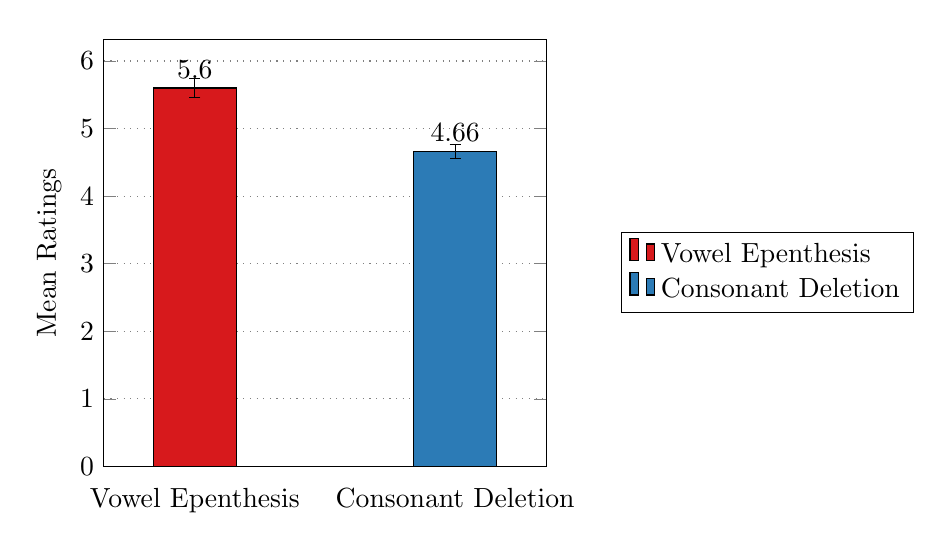
\begin{tikzpicture}
  \begin{axis}[
  ylabel={Mean Ratings},
width=7.2cm,
   height = 7cm,
    ytick distance=1,
        nodes near coords,
      major x tick style = transparent,
    ybar=3*\pgflinewidth,
      bar width=30pt,
      ymajorgrids = true,
      symbolic x coords={Vowel Epenthesis,Consonant Deletion},
      xtick ={Vowel Epenthesis, Consonant Deletion},
      scaled y ticks = false,
        legend style={at={(1.5,0.55)},
  anchor=north},
  legend cell align=left,
      enlarge x limits=0.35,
      ymin=0,
       every axis plot/.append style={
          ybar,
          bar shift=0pt,
          fill
        }
    ]

 \addplot [fill=mycolor1,error bars/.cd, y dir=both, y explicit,error bar style=black] 
  coordinates {
          (Vowel Epenthesis, 5.60) += (0,0.14) -= (0,0.14)};
\addplot [fill=mycolor4,error bars/.cd, y dir=both, y explicit,error bar style=black] 
  coordinates {
          (Consonant Deletion, 4.66) += (0,0.10) -= (0,0.10)};
 \legend{Vowel Epenthesis,Consonant Deletion}
 \end{axis}
\end{tikzpicture}
\end{center}
\end{block}
}

\end{frame}
%-----------------------------------------------
\subsection{summary}
\begin{frame}
\frametitle{Summary}
\begin{itemize}
\onslide<1->{\item Consonant errors in L2 are more accented than syllable and vowel errors.\linebreak}
\onslide<2->{\item Phonological environments affect accentedness perception.
\onslide<3-> \item[1] English phonotactics (Probability of sound/feature combinations in native speech)
\onslide<4->\item[2] Prosodic environment (e.g. Domain-initial v.s. domain medial)
\onslide<5->\item[3] Acoustic similarities (e.g. sonority profile, /\textipa{T}/ v.s. /f/ v.s. /t/)
}
\end{itemize}
\end{frame}

%------------------------------------------------
\begin{frame}
\frametitle{Future Directions}
\begin{itemize}
\onslide<1->{\item The relationship between accentedness and {\bf English phonotactics} and {\bf acoustic similarities} }\linebreak
\onslide<2->{\item Methodological issues
\onslide<3-> \item[1] The necessity of presenting orthography
\onslide<4->\item[2] The necessity of training sessions 
}
\end{itemize}
\end{frame}
%------------------------------------------------

%------------------------------------------------
\section{References}
\begin{frame}[shrink=20]
\frametitle{References}
\footnotesize{
\begin{itemize}
\item Chan, K. Y., Hall, M. D., \& Assgari, A. A. (2016). The role of vowel formant frequencies and duration in the perception of foreign accent. \emph {Journal of Cognitive Psychology}, 1\textendash{}12.
\item Hayes, B., \& Wilson, C. (2008). A maximum entropy model of phonotactics and phonotactic learning. \emph{Linguistic inquiry}, 39(3), 379-440.
\item Magen, H. S. (1998). The perception of foreign-accented speech. \emph{Journal of Phonetics}, 26(4), 381\textendash{}400.
\item Major, R. C. (1987). Phonological similarity, markedness, and rate of L2 acquisition. \emph{Studies in Second Language Acquisition}, 9(01), 63\textendash{}82.
\item Morrill, T., \& Gao, Z. (2016). Discriminability of non-native tonal contours in low-pass filtered speech. \emph{The Journal of the Acoustical Society of America}, 139(4), 2162-2163.
\item McCullough, E. A. (2013). \emph{Acoustic correlates of perceived foreign accent in non-native English}. The Ohio State University (Doctorate Dissertation). 
\item Solon, M. (2015). L2 Spanish/l: The Roles of F2 and Segmental Duration in Foreign Accent Perception. \emph{In Selected Proceedings of the 6th Conference on Laboratory Approaches to Romance Phonology} (pp. 83\textendash{}94). 
\item Van Den Doel, R. (2006). \emph{How friendly are the natives? An evaluation of native-speaker judgements of foreign-accented British and American English }(Doctoral dissertation, Netherlands Graduate School of Linguistics).
\item Weinberger, S. H. (2016). \emph{Speech accent archive }[Database]. Retrieved from http://accent.gmu.edu
\item Wilson, C., \& Davidson, L. (2013). Bayesian analysis of non-native cluster production. \emph{In Proceedings of NELS (Vol. 40).} 
\item Steinschneider, M.; Volkov, I. O.; Noh, M. D.; Garell, P. C.; Howard Ma, 3. (1999). Temporal encoding of the voice onset time phonetic parameter by field potentials recorded directly from human auditory cortex. \emph{Journal of Neurophysiology}. 82 (5): 2346–2357.

\end{itemize}}
\end{frame}
%------------------------------------------------

%------------------------------------------------

\begin{frame}
\Huge{\centerline{Thank You!}}
\end{frame}

%----------------------------------------------------------------------------------------

%----------------------------------------------------------------------------------------
\section{Supplemental Materials}
\subsection{Ratings}
\begin{frame}
\frametitle{Supplemental Materials \Romannum{1}: Ratings}
\only <1>{
\begin{block}{ask her}
\begin{figure}
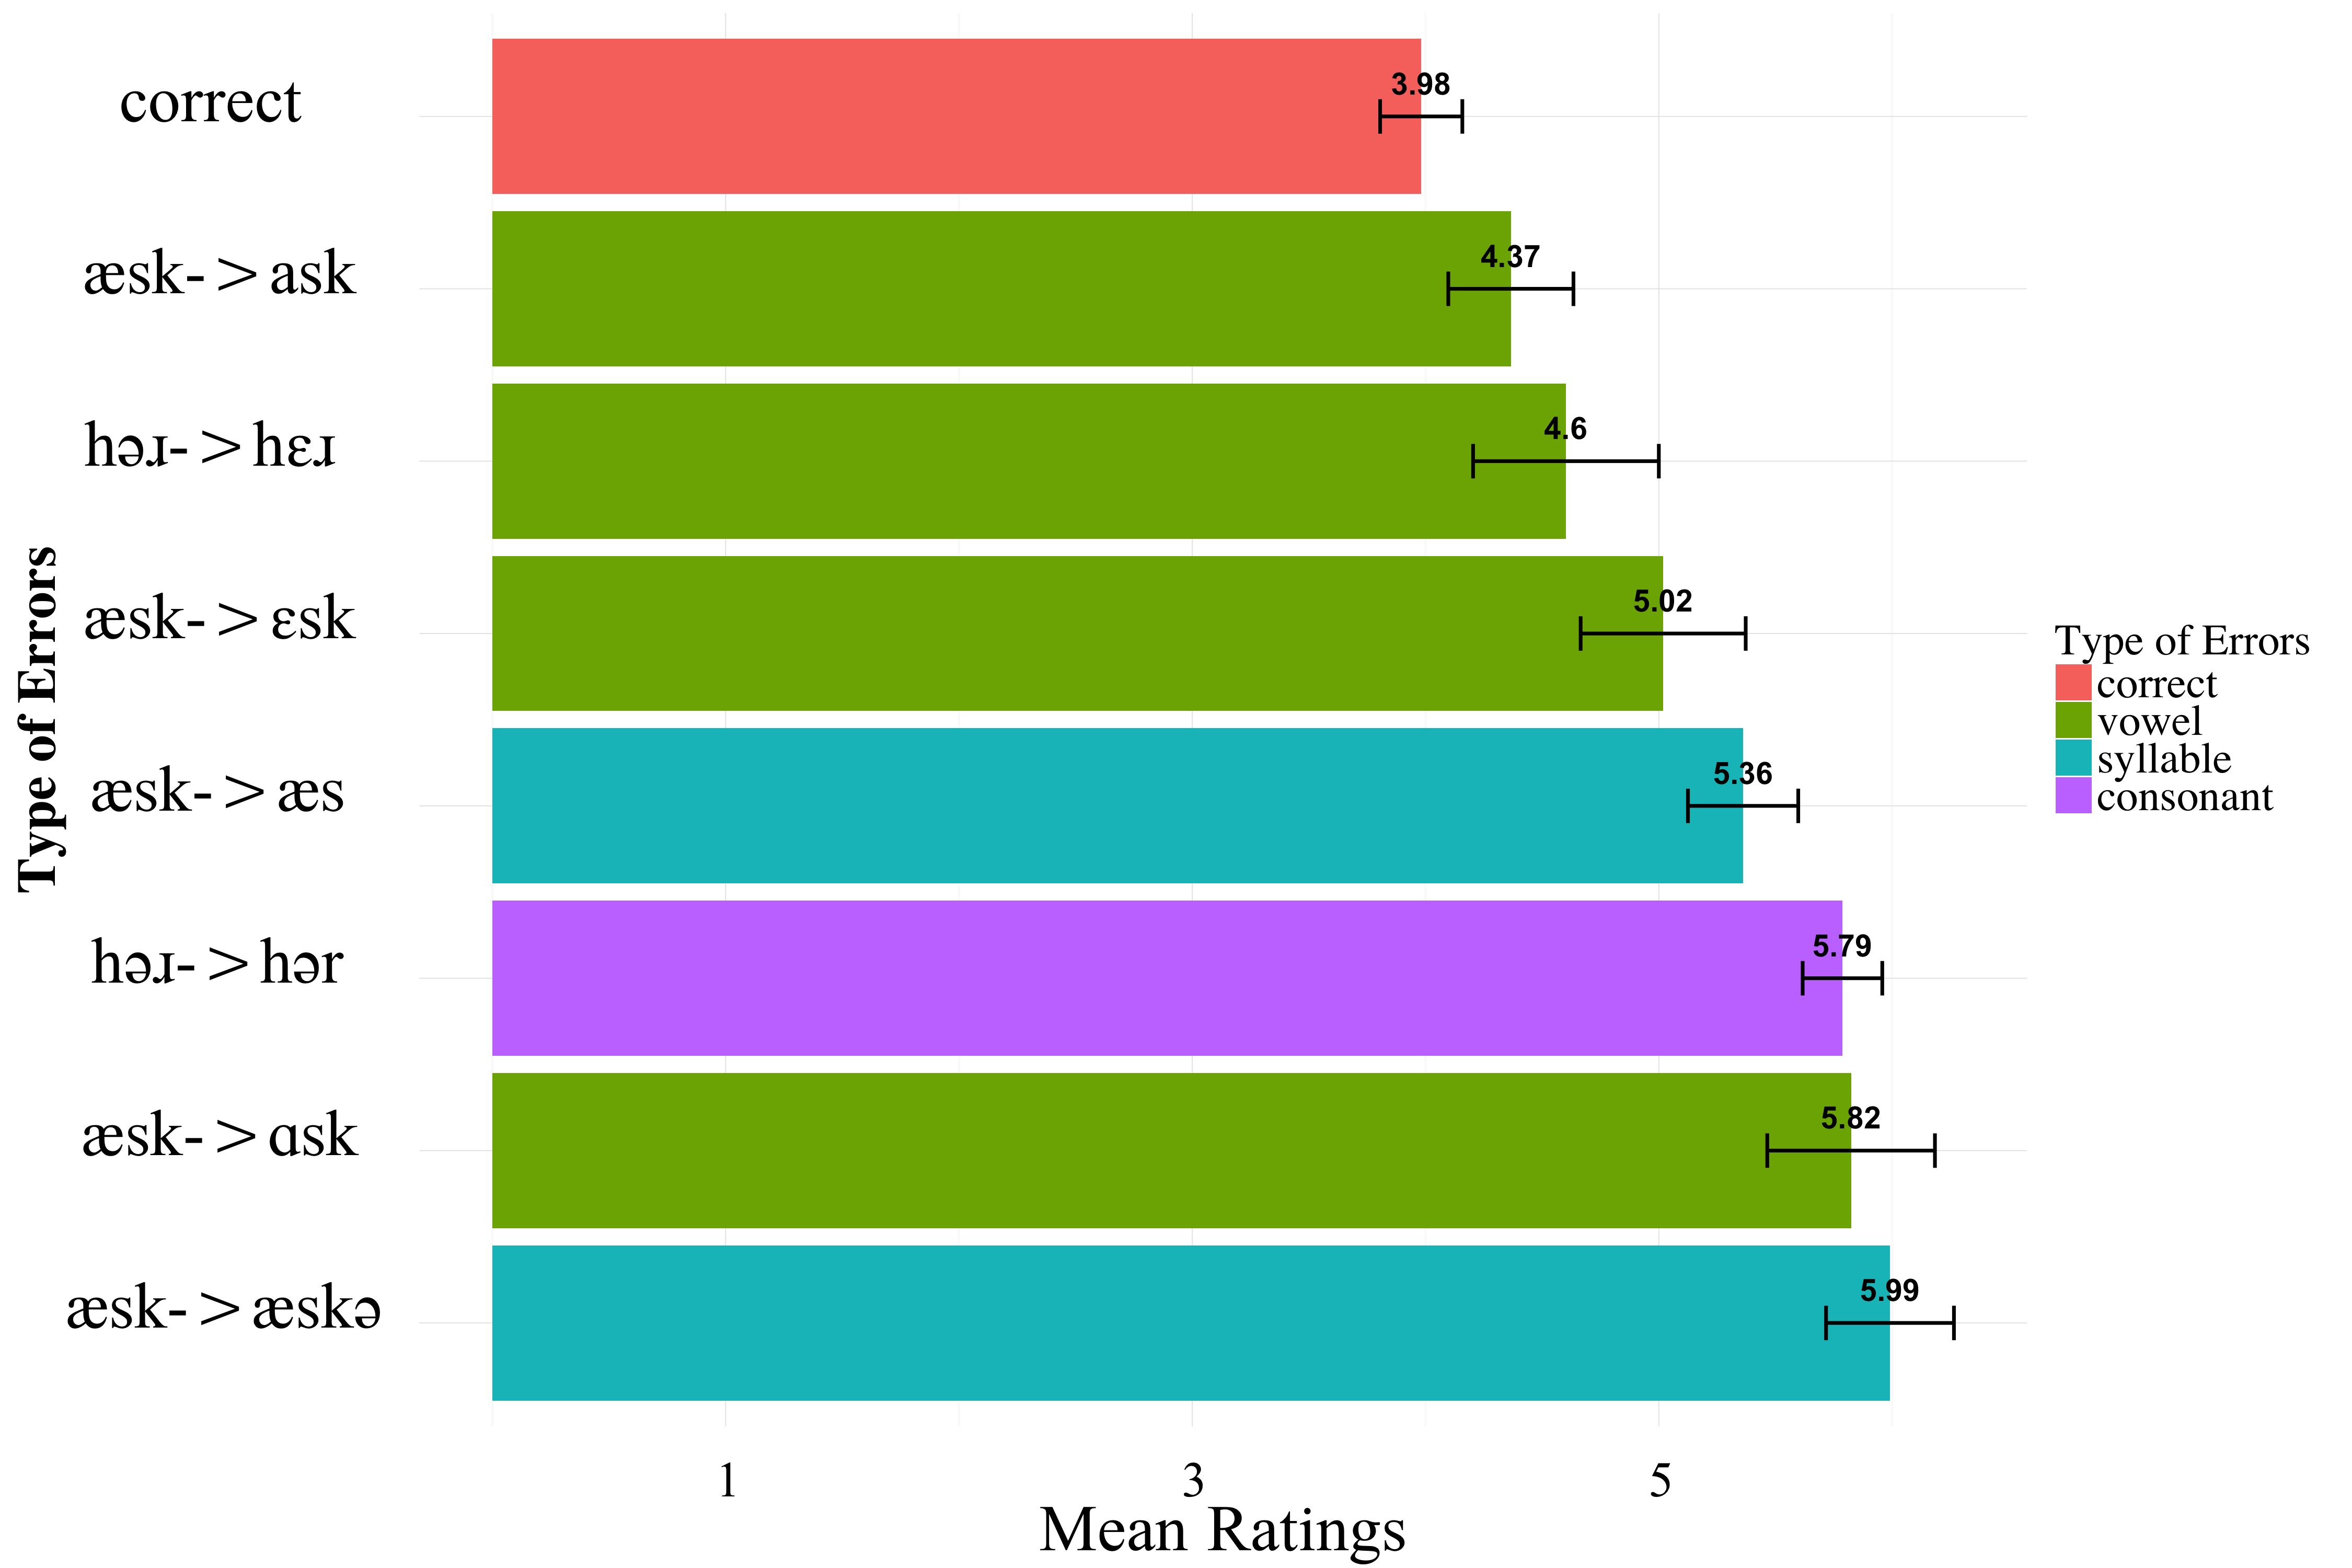
\includegraphics[width=0.8\linewidth]{ak_detailed}
\end{figure}
\end{block}}
\only <2>{
\begin{block}{six spoons}
\begin{figure}
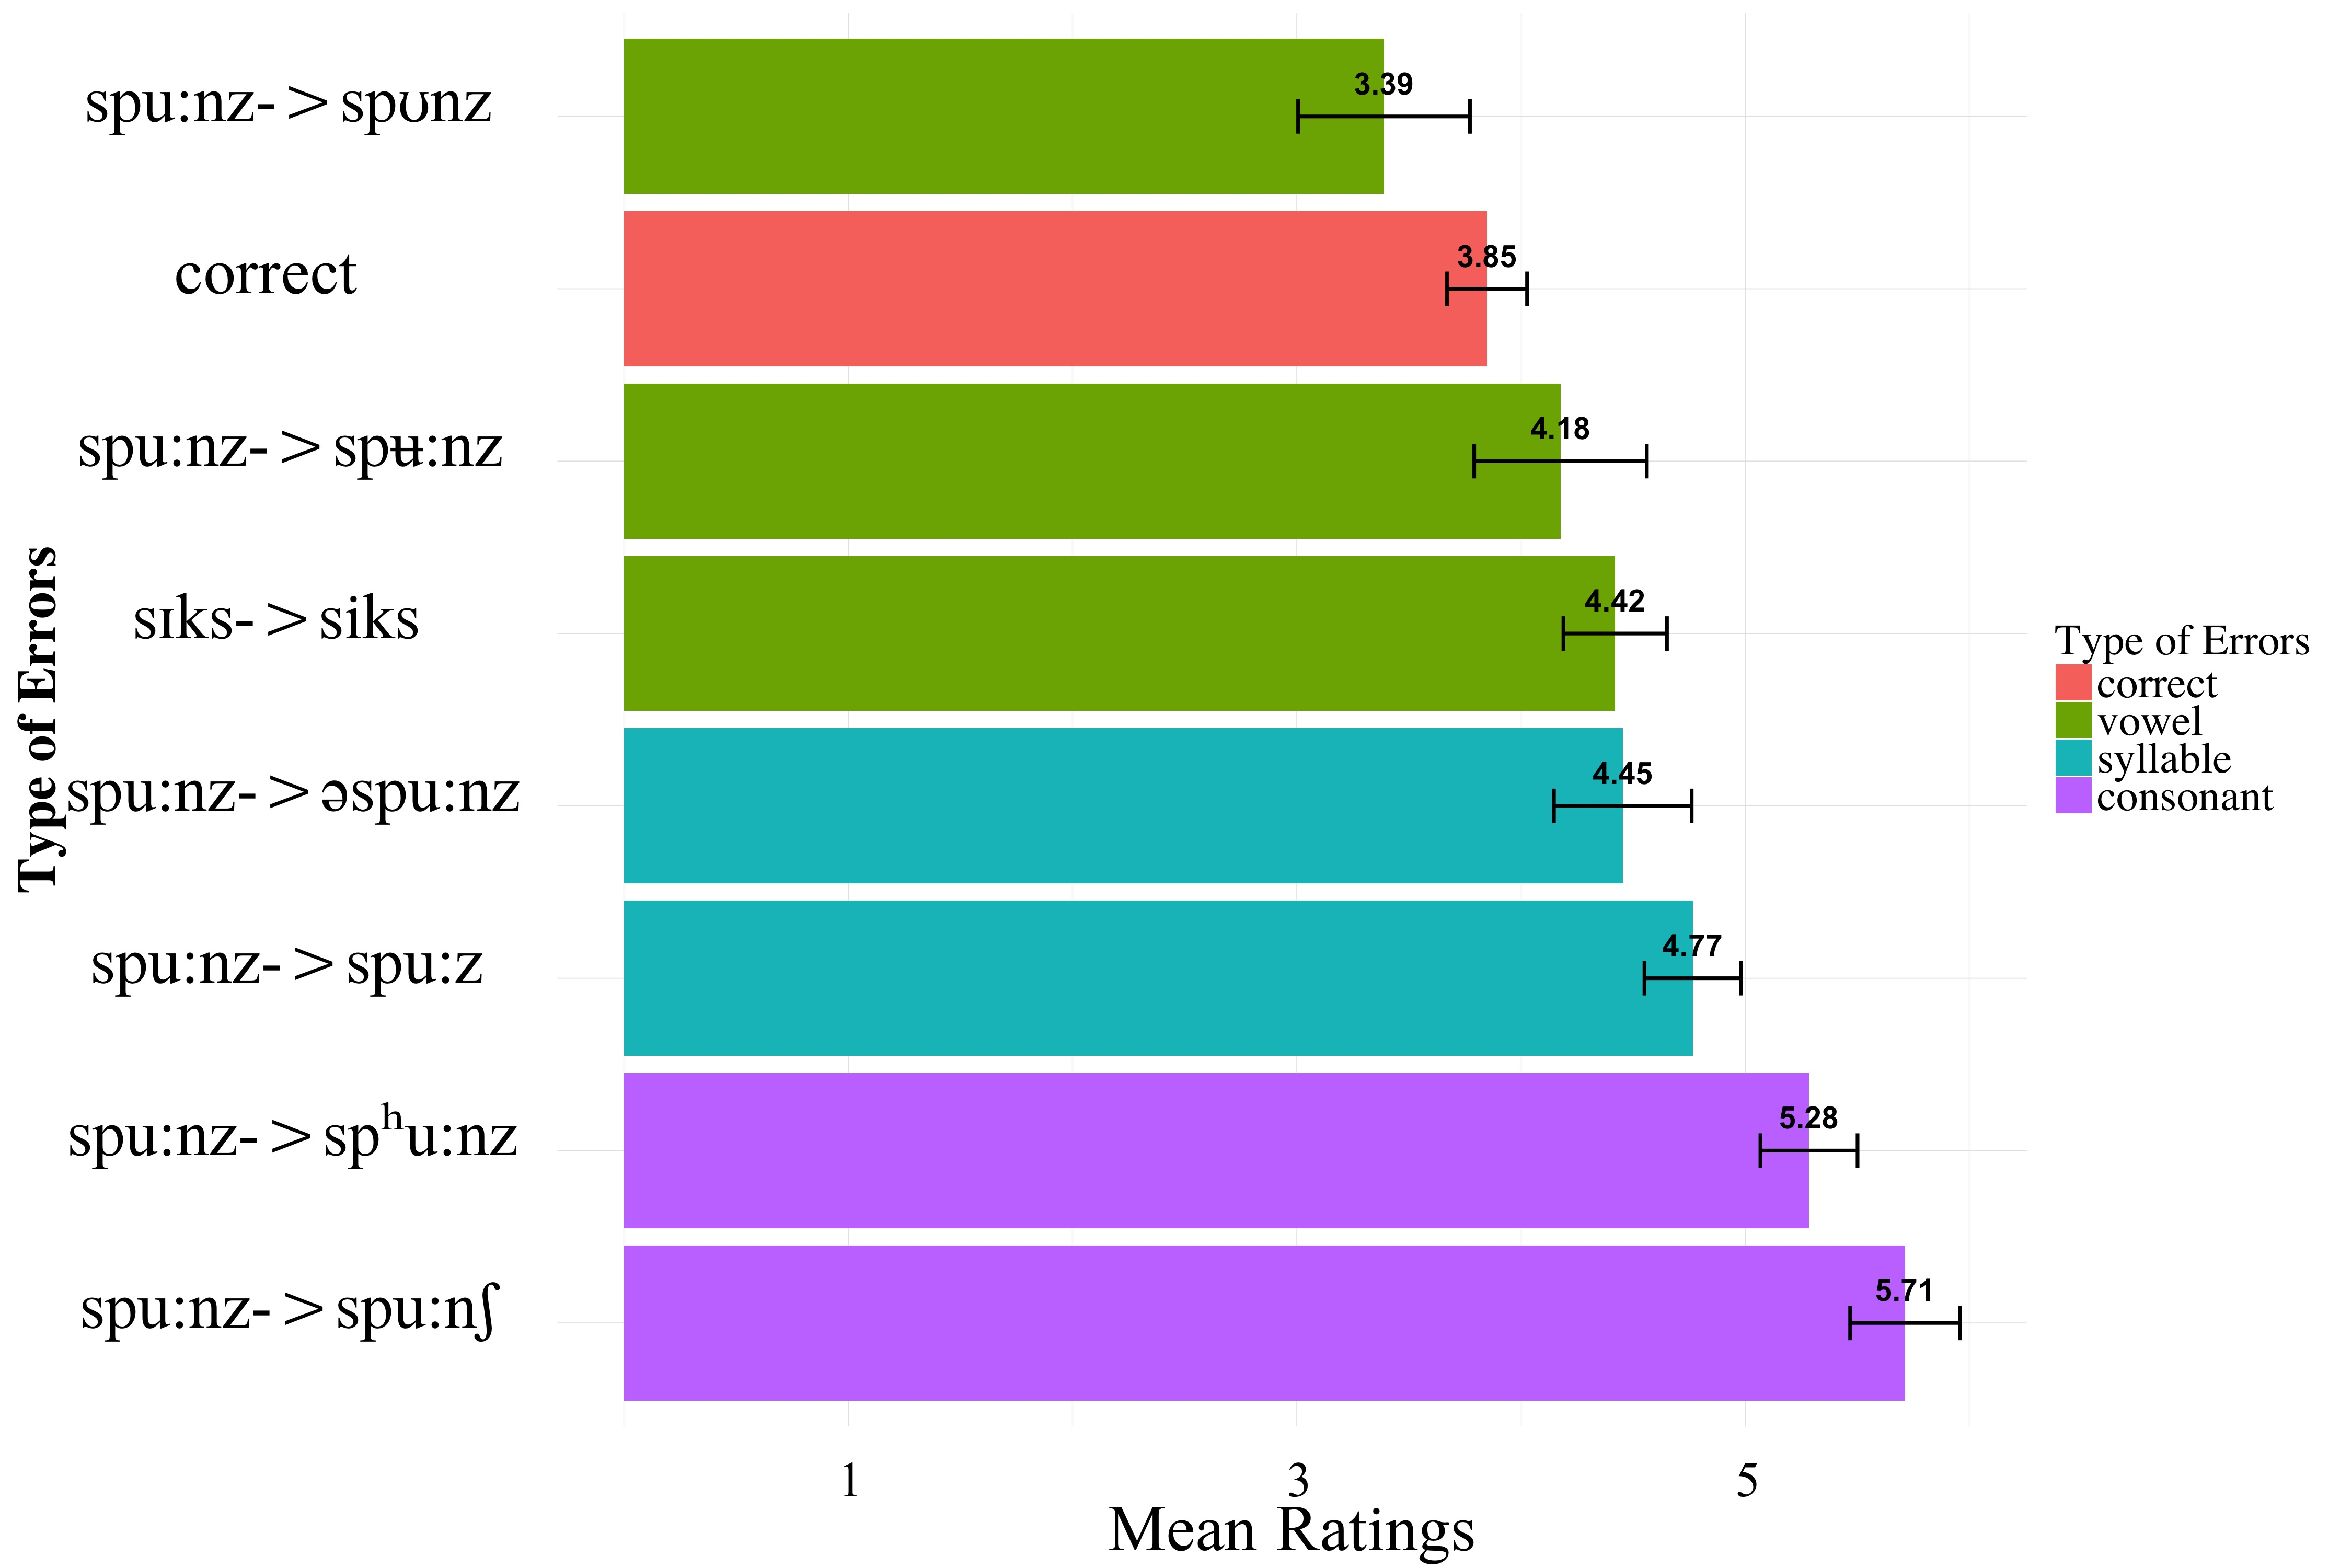
\includegraphics[width=0.8\linewidth]{ss_detailed}
\end{figure}
\end{block}}
\only <3>{
\begin{block}{please call}
\begin{figure}
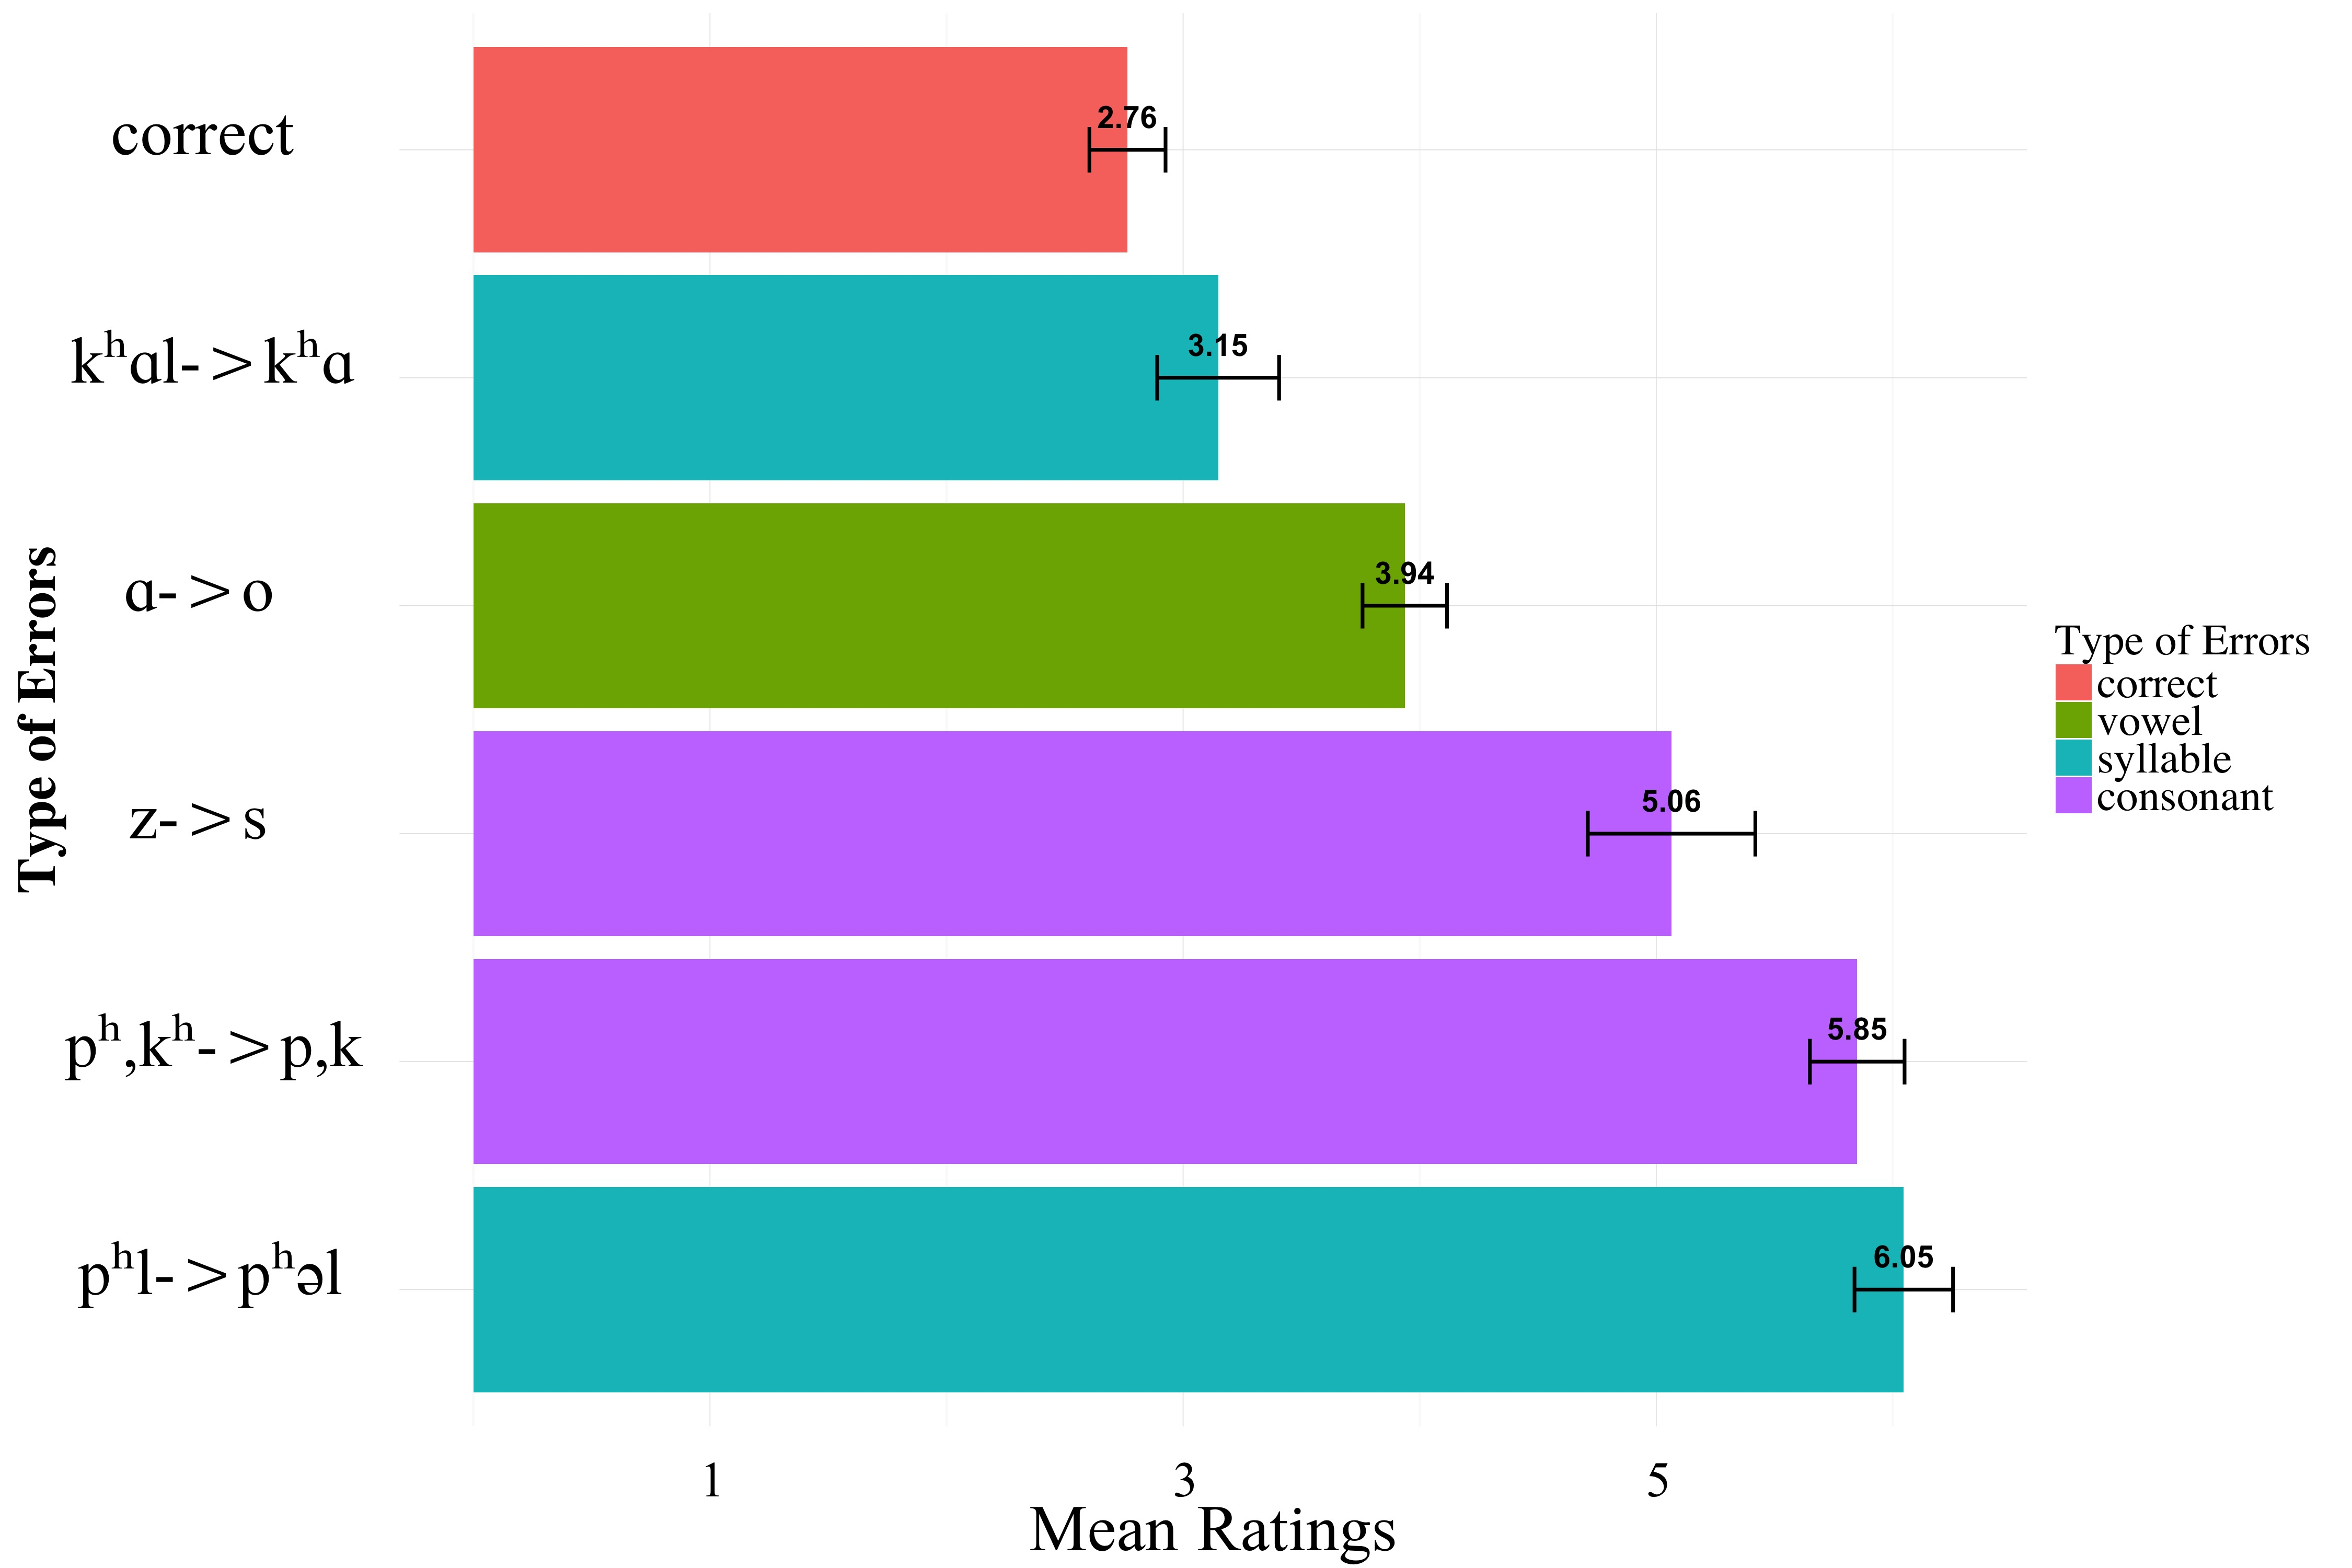
\includegraphics[width=0.8\linewidth]{pc_detailed}
\end{figure}
\end{block}}
\only <4>{
\begin{block}{small plastic}
\begin{figure}
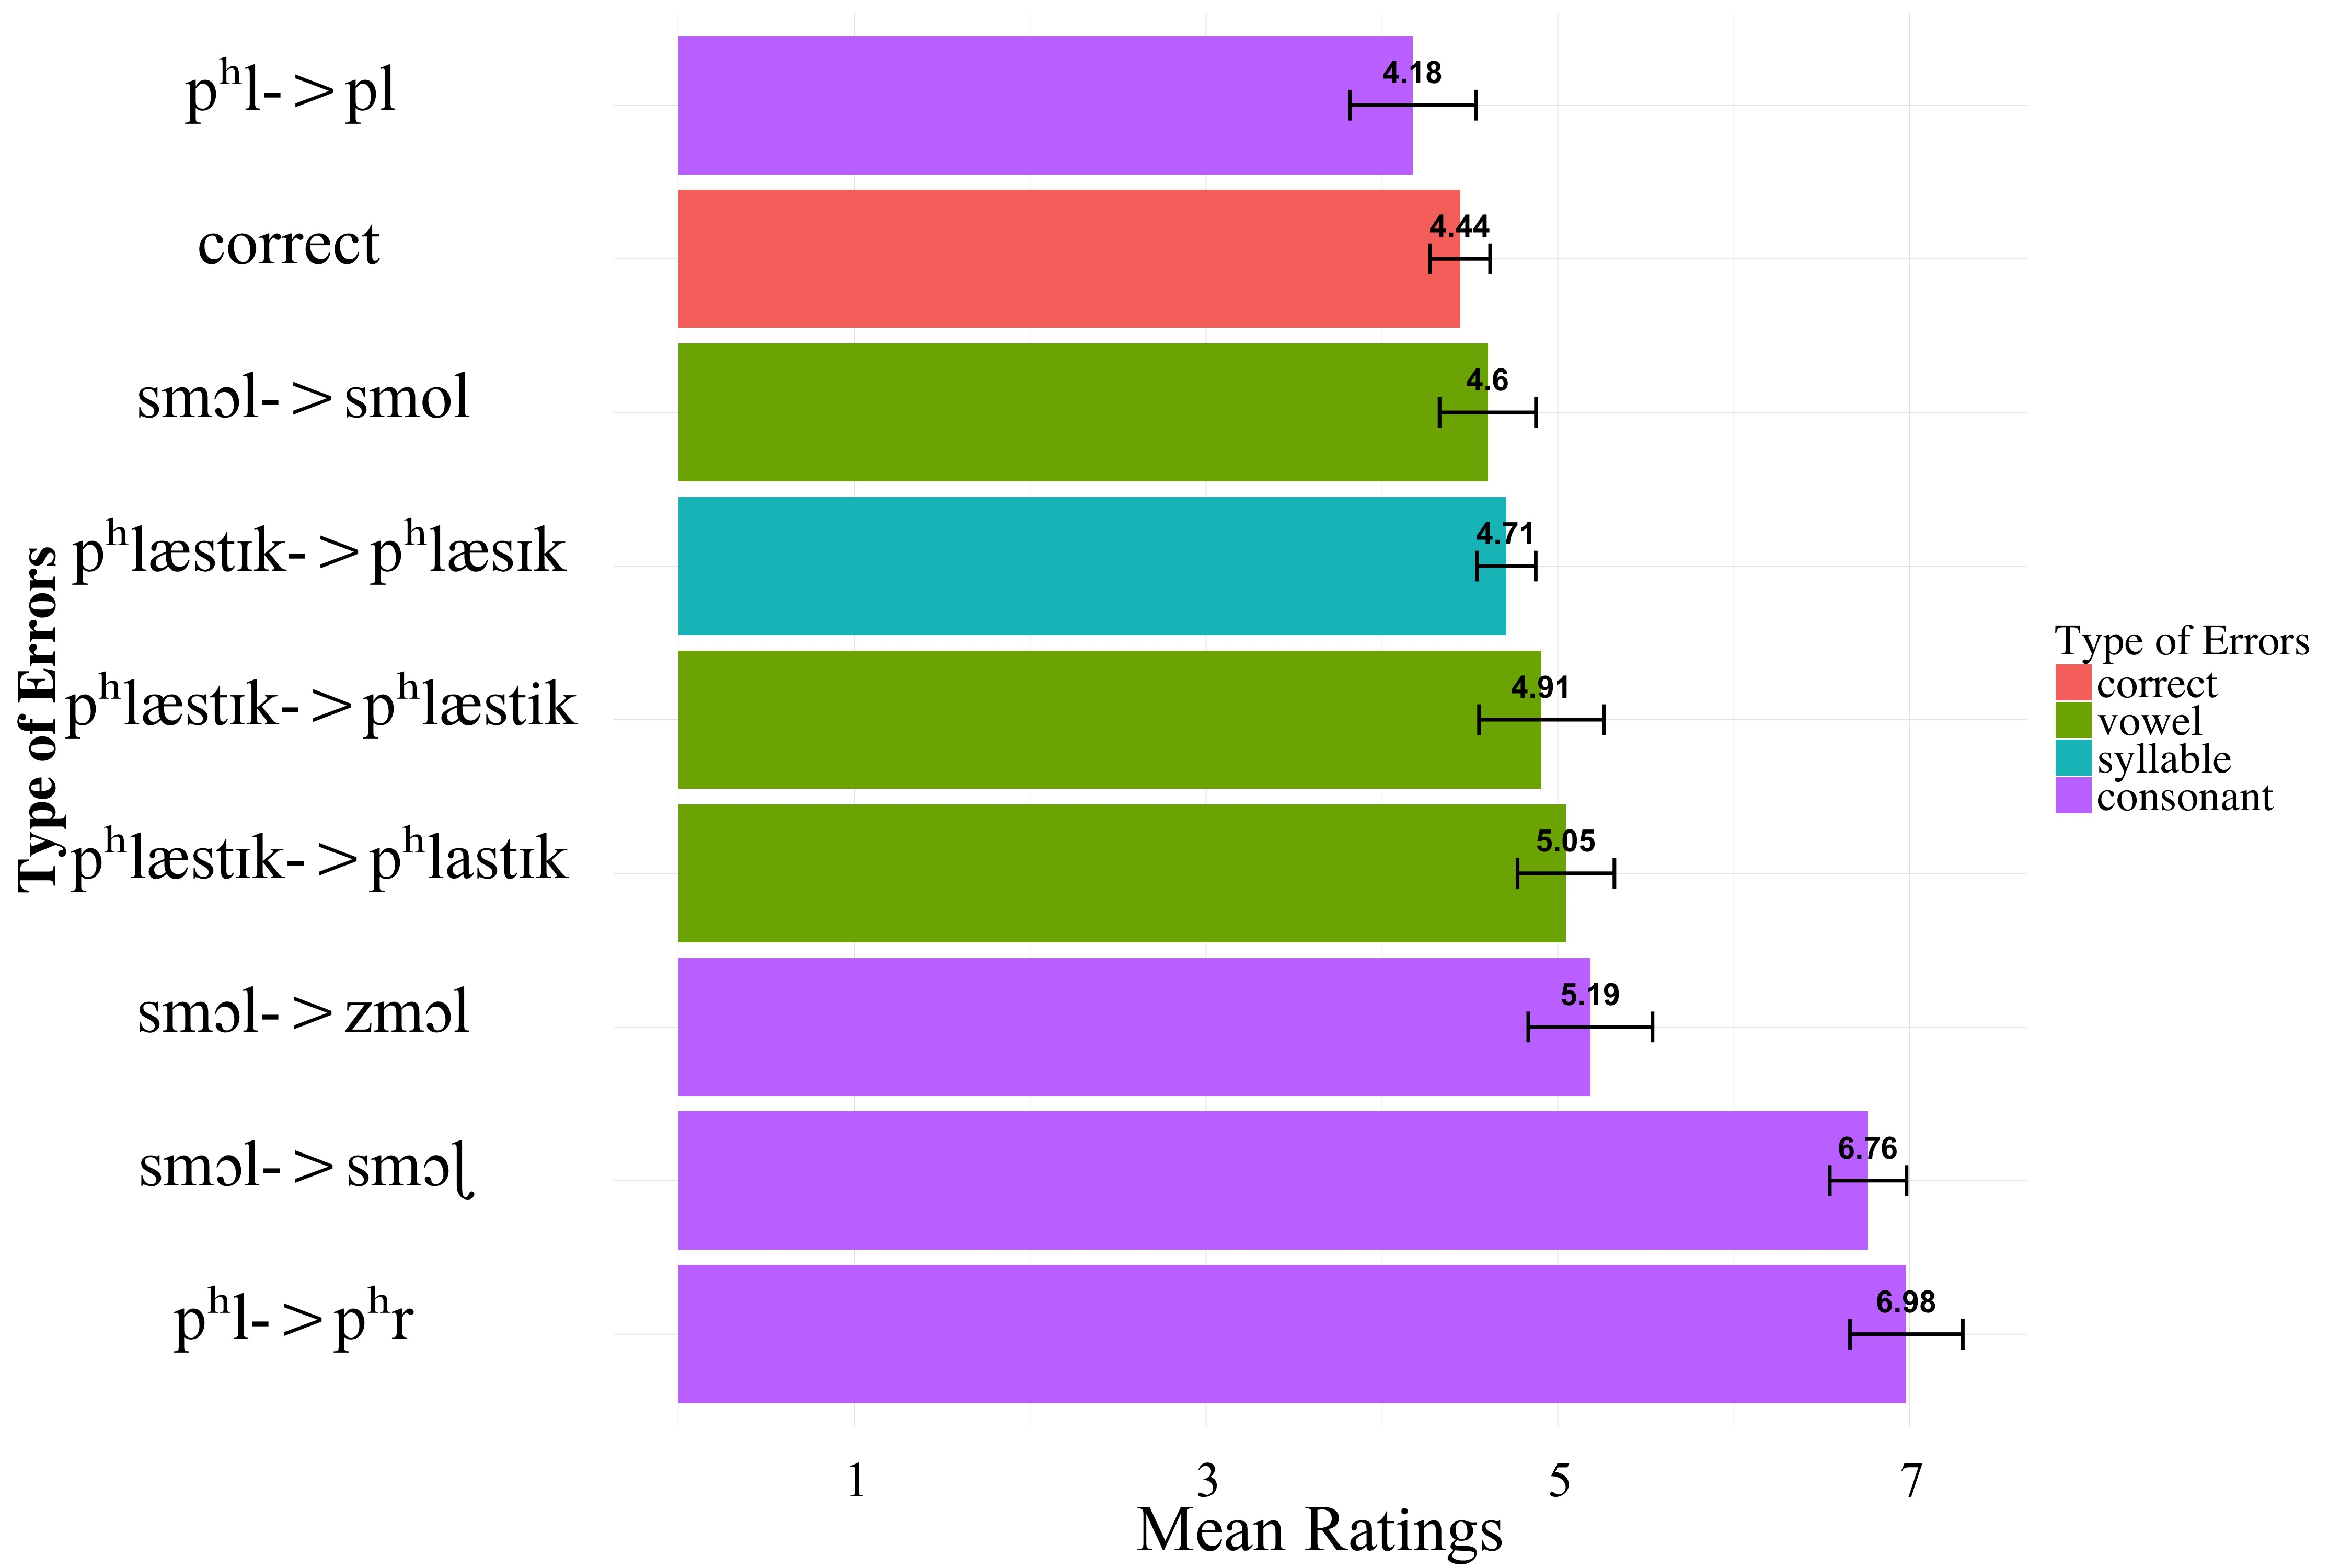
\includegraphics[width=0.8\linewidth]{sp_detailed}
\end{figure}
\end{block}}
\end{frame}
%--------------------
\subsection{NLs}
\begin{frame}
\frametitle{NLs}
\begin{figure}
\includegraphics[width=0.8\linewidth]{l1}
\end{figure}
\end{frame}
\subsection{Type of errors}
\begin{frame}
\frametitle{Type of Errors:Consonant}
\begin{figure}
\includegraphics[width=0.8\linewidth]{error1}
\end{figure}
\end{frame}
\subsection{Type of errors2}
\begin{frame}
\frametitle{Type of Errors}
Vowel
\begin{figure}
\includegraphics[width=0.8\linewidth]{error2}
\end{figure}
Syllable
\begin{figure}
\includegraphics[width=0.8\linewidth]{error3}
\end{figure}
\end{frame}
\subsection{Countries}
\begin{frame}
\frametitle{L1s of the talkers}
\begin{figure}
\includegraphics[width=0.8\linewidth]{countries}
\end{figure}
\end{frame}
%--------------------
\subsection{MaxEnt}
\begin{frame}
\frametitle{The current study \Romannum{2}: Data Analysis}
Maximum Entropy as Well-formedness \textsubscript{(Hayes \& Wilson, 2008)}\linebreak
\begin{table}[]
\caption{Pilot study-- Well-formedness of Mandarin accent}
\label{my-label}
\begin{tabular}{lllll}
\toprule
       & \textsubscript{\bf *{[}+continuant{]}{[}+voice,-coronal{]} }&....&  \textsubscript{\bf *{[}+voice{]}{[}-coronal{]}} & MaxEnt \\
 \midrule
sm  &      \multicolumn{1}{c}{0.179}            &  ...          &  \multicolumn{1}{c}{0}   &  \multicolumn{1}{c}{1.619}      \\
\textipa{S}m & \multicolumn{1}{c}{0.179}          & ...           &\multicolumn{1}{c}{0}       & \multicolumn{1}{c}{\color{red}10.648}       \\
\textipa{\:s}m & \multicolumn{1}{c}{0.179}          & ...           &\multicolumn{1}{c}{0}       & \multicolumn{1}{c}{\color{red}11.224}       \\
\textipa{C}m &       \multicolumn{1}{c}{0.179}   & ...           & \multicolumn{1}{c}{0}      & \multicolumn{1}{c}{\color{red}11.712}     \\
zm & \multicolumn{1}{c}{0.179}	&...	&\multicolumn{1}{c}{1.021}	&\multicolumn{1}{c}{\color{red}13.893}	\\
\bottomrule
\end{tabular}
\end{table}
\textsubscript{L2 data: GMU Speech Accent Archive}\linebreak
\textsubscript{English data: CMU Sphinx Dictionary}
\end{frame}
%-------------------
\subsection{Predictions}
\begin{frame}
\frametitle{The current study \Romannum{3}: Predictions}
\begin{block}{Ranking of Errors}
\begin{figure}
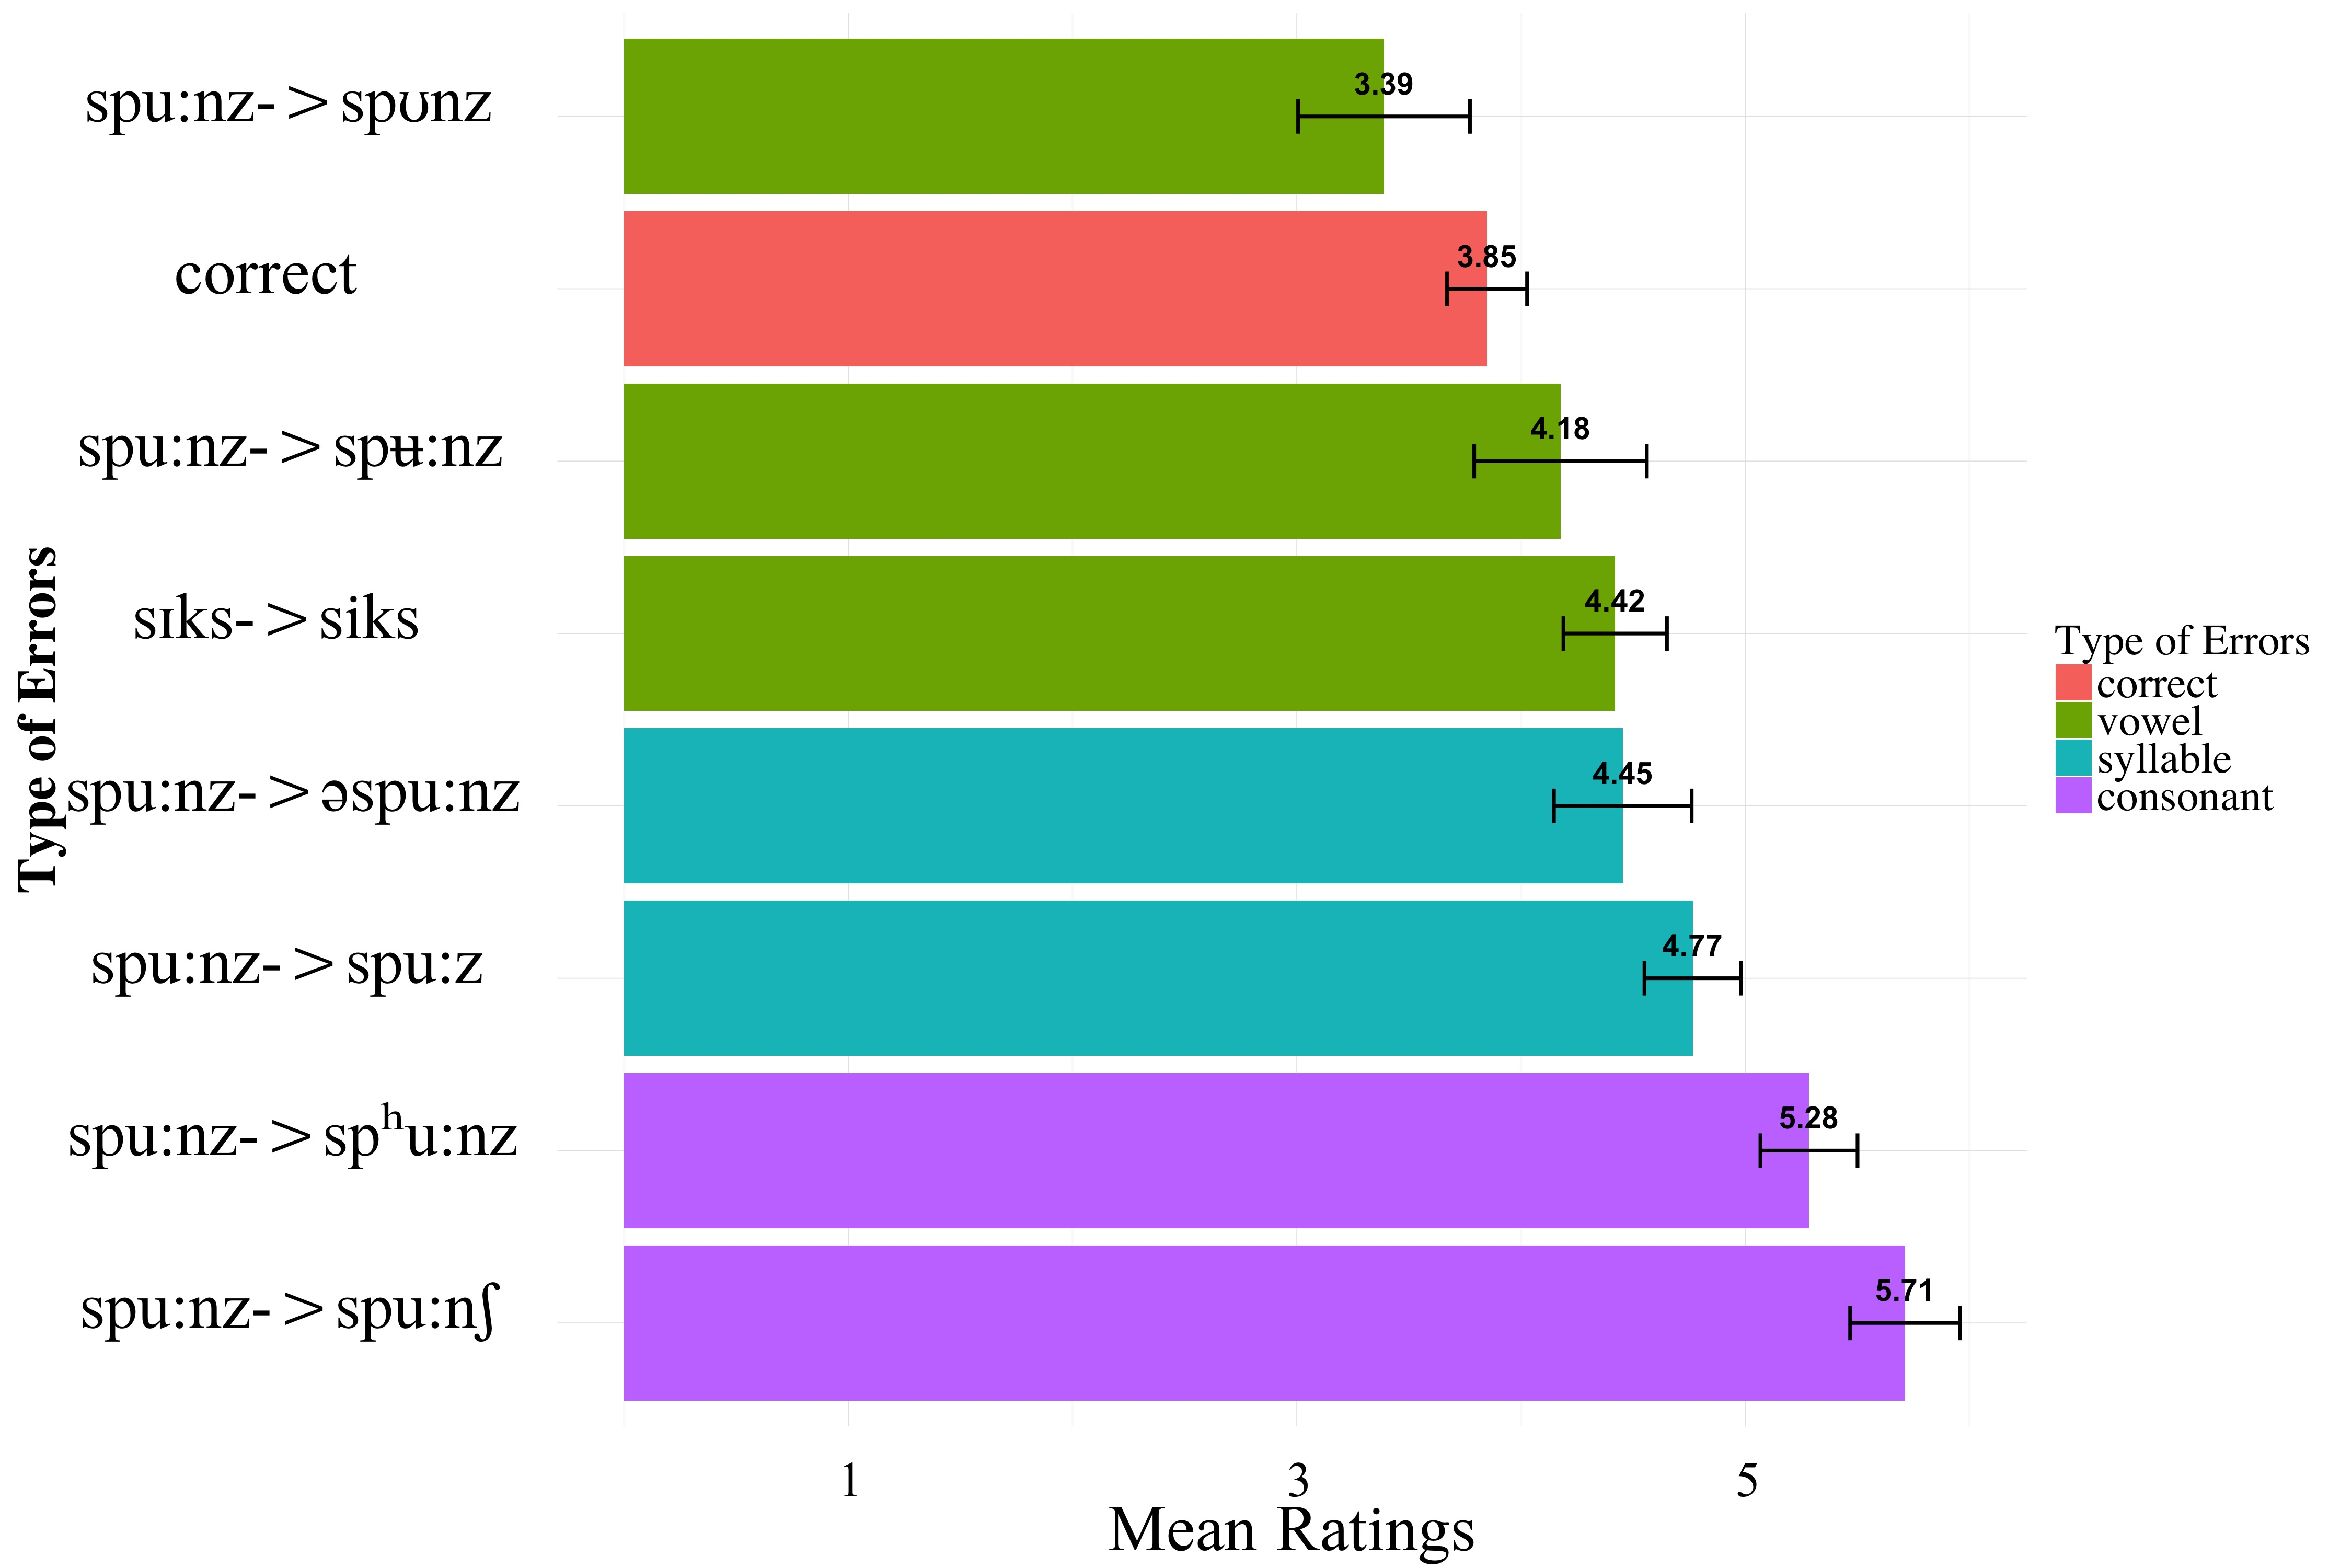
\includegraphics[width=0.8\linewidth]{ss_detailed}
\end{figure}
\end{block}
\end{frame}
\begin{frame}
\frametitle{The current study \Romannum{3}: Predictions}
\begin{block}{Well-formedness \& Accentedness}
\begin{figure}
\includegraphics[width=0.8\linewidth]{red}
\end{figure}
\end{block}
\end{frame}
%-------------------
\subsection{Choropleth Map}
\begin{frame}
\frametitle{Supplemental materials \Romannum{2}:Ratings by State }
\begin{figure}
\includegraphics[width=0.9\linewidth]{heat}
\end{figure}
\end{frame}
%-----------------
\subsection{MaxEnt Constraints}
\begin{frame}
\frametitle{Supplemental materials \Romannum{3}:MaxEnt Constraints}
\begin{table}[]
\begin{tabular}{ll}
*{[}-sonorant,+continuant,+voice,+distributed{]}                  & 2.277 \\
*{[}+nasal,+DORSAL{]}                                             & 2.489 \\
*{[}-anterior,-distributed{]}                                     & 4.448 \\
*{[}-sonorant,-back{]}                                            & 3.986 \\
*{[}+voice{]}{[}-approximant{]}                                   & 0.349 \\
*{[}-word\_boundary{]}{[}+delayedRelease{]}                       & 4.571 \\
*{[}-CORONAL{]}{[}-approximant{]}                                 & 5.217 \\
*{[}-continuant{]}{[}-approximant{]}                              & 2.355 \\
*{[}-word\_boundary{]}{[}-sonorant,+voice{]}                      & 2.312 \\
*{[}+distributed{]}{[}+consonantal{]}                             & 2.15  \\
*{[}+continuant,+voice{]}{[}-word\_boundary{]}                    & 2.229 \\
*{[}+distributed{]}{[}-CORONAL{]}                                 & 0.921 \\
*{[}+sonorant{]}{[}-word\_boundary{]}                             & 5.019 \\
*{[}+LABIAL{]}{[}-CORONAL{]}                                      & 4.001 \\
\vdots & \vdots \\
\end{tabular}
\end{table}
\end{frame}

\end{document}